% \iffalse meta-comment
%<=*COPYRIGHT>
%% Copyright (C) 2009-2012 by Martin Scharrer <martin@scharrer-online.de>
%% ----------------------------------------------------------------------
%% This work may be distributed and/or modified under the
%% conditions of the LaTeX Project Public License, either version 1.3
%% of this license or (at your option) any later version.
%% The latest version of this license is in
%%   http://www.latex-project.org/lppl.txt
%% and version 1.3 or later is part of all distributions of LaTeX
%% version 2005/12/01 or later.
%%
%% This work has the LPPL maintenance status `maintained'.
%%
%% The Current Maintainer of this work is Martin Scharrer.
%%
%% This work consists of the files tikz-timing.dtx and tikz-timing.ins
%% and the derived filebase tikz-timing*.sty.
%%
%<=/COPYRIGHT>
% \fi
%
% \iffalse
%<*driver>
\ProvidesFile{tikz-timing.dtx}[%
%<=*DATE>
    2011/01/09
%<=/DATE>
%<=*VERSION>
    v0.7d
%<=/VERSION>
    DTX-File of 'tikz-timing' package.]
\newif\ifprintversion % \fi
\ifdefined\printversion
  \printversiontrue
\fi

\RequirePackage{filecontents}
\begin{filecontents}{ydoc.cfg}
  % Intensionally empty
\end{filecontents}

\ifprintversion
  \documentclass{ltxdoc}
  \let\chapter\section
  \let\section\subsection
  \let\subsection\subsubsection
\else
  \documentclass[landscape,12pt]{scrreprt}
  \usepackage{ydoc}
\fi
\GetFileInfo{tikz-timing.dtx}
\usepackage{tikz-timing}[\filedate]

\usepackage{hyperref}
\usepackage{atbegshi}
\usetikztiminglibrary{arrows,either,overlays,clockarrows,columntype}
\usetikztiminglibrary{nicetabs,counters,advnodes,interval,ifsym}
\tikzset{timing/no nice tabs}
\tikzset{timing/interval/normal}
\tikzset{timing/nodes/old center}
\usetikzlibrary{plotmarks}
\makeatother
%%%^^A\usepackage[electronic]{ifsym}
\usepackage{calc}
\usepackage{graphicx}
\usepackage{xcolor}
\usepackage{tabularx}
\usepackage{array}
\usepackage{flafter,fnpos}
\usepackage{booktabs}
\usepackage{supertabular}
%\usepackage{xtab}
\usepackage{amsmath}
\usepackage{flafter}
\usepackage{placeins}
\makeFNbottom
\makeFNbelow
\usepackage{microtype}[2005/10/28]
\DisableLigatures{encoding = T1, family = tt* }%
\newsavebox{\mysb}
\newsavebox{\sba}
\newsavebox{\sbb}

\def\topfraction{0.91}
\def\bottomfraction{0.95}
\def\floatpagefraction{0.98}
\def\textfraction{0.05}
\setcounter{bottomnumber}{2}

\usepackage{listings}
\lstset{basicstyle=\ttfamily}

\usepackage{shortvrb}
\usepackage{newverbs}
\MakeSpecialShortVerb{\qverb}{\"}

\def\NewIn#1{
  \marginpar{\strut\raggedleft\raisebox{.125ex}{\textcolor{black}{\emph{New in #1}}}}%
}

\def\ExtIn#1{
  \marginpar{\strut\raggedleft\textcolor{black}{\emph{Extended in #1}}}%
}

\iffalse
\def\thesection{\texorpdfstring{\LARGE\texttiming[X]{D{\arabic{section}}.1X[black]}}{\arabic{section}}}
\def\thesubsection{\texorpdfstring{\Large\texttiming[X]{D{\arabic{section}}D{\arabic{subsection}}.1X[black]}}{\arabic{section}.\arabic{subsection}}}
\def\thesubsubsection{\texorpdfstring{\large\texttiming[X]{D{\arabic{section}}D{\arabic{subsection}}D{\arabic{subsubsection}}.1X[black]}}
{\arabic{section}.\arabic{subsection}.\arabic{subsubsection}}}

 %\def\timingsectionformat#1{%
 %  \sbox{\mysb}{\tikz \draw node [timing/d/text] {#1};}%
 %  \texttiming{ $ \wd\mysb / \tikztiming@xunit $ DD{#1} }%
 %}

\renewcommand\section{\@startsection {section}{1}{\z@}%
                                   {-3.5ex \@plus -1ex \@minus -.2ex}%
                                   {2.3ex \@plus.2ex}%
                                   {\normalfont\Large\bfseries\sffamily}}
                                   %[#1]{\texorpdfstring{\larger\timingsectionformat{#2}}{#2}}}
\renewcommand\subsection{\@startsection{subsection}{2}{\z@}%
                                     {-3.25ex\@plus -1ex \@minus -.2ex}%
                                     {1.5ex \@plus .2ex}%
                                     {\normalfont\large\bfseries\sffamily}}
\renewcommand\subsubsection{\@startsection{subsubsection}{3}{\z@}%
                                     {-3.25ex\@plus -1ex \@minus -.2ex}%
                                     {1.5ex \@plus .2ex}%
                                     {\normalfont\normalsize\bfseries\sffamily}}
\fi

\let\envv\env
\let\css\cs
\def\lib{\texttt}
\def\library#1#2{\section{#2}\label{lib:#1}}

\usepackage{xspace}
\def\ie{i.e.\xspace}
\def\eg{e.g.\xspace}

\makeatletter
% The following code is only needed to produce package examples and therefor not 
% included in the style file but might be written to an additional file.
% \iffalse
%</driver>
%<*examplecode>
% \fi
%
% \begin{environment}{tikztimingexampletable}
%    \begin{macrocode}
\newenvironment{tikztimingexampletable}{%
  \begingroup
  \let\tikztimingtable@row\tikztimingexampletable@row
  \tikzset{timing/nice tabs}
  \tikztimingtable
}{%
  \extracode
    \tableheader{Characters}{Resulting Diagram}%
    \tablerules
\endtikztimingtable
\endgroup
}%
%    \end{macrocode}
% \end{environment}
%
% \begin{macro}{\tikztimingexampletable@row}[1]{Row content}
%    \begin{macrocode}
\long\def\tikztimingexampletable@row#1\\{%
  \def\tikztiming@text{#1}%
  \@onelevel@sanitize\tikztiming@text
  \tikztimingtable@row@@{\ttfamily\tikztiming@text}{#1}%
}
%    \end{macrocode}
% \end{macro}
%
% \begin{macro}{\tikztimingfullexampletable}
%    \begin{macrocode}
\def\tikztimingfullexampletable{%^^A
  \begin{tikzpicture}[timing/picture,x=1em,y=1em,font=\sffamily]
    \tikzset{timing/d/background/.style={fill={gray!25},fill opacity=0.5}}%
    \let\chars\tikztiming@chars@default
    \node (charnode) at (0,0) {%
       \scalebox{0.4}%
         {\rotatebox{-45}{$\frac{\mbox{\rotatebox{45}{to}}}%
         {\mbox{\rotatebox{45}{from}}}$}}%
    };
    \coordinate (charnodex) at (0.25,0);%
    \coordinate (charnodey) at (0,0);%
    \expandafter\foreach
    \expandafter\tchar
    \expandafter i\expandafter n\expandafter{\chars} {%
      \path (charnodex) ++(+2,0) node (charnodex) {\strut\tchar};
      \path (charnodey) ++(0,-2) node (charnodey) {\strut\tchar};
    }%
    \draw [line width=\heavyrulewidth] (charnodex) +(+1,+1) -- (-1,+1);
    \draw [line width=\lightrulewidth]  (charnodex) +(+1,-1) -- (-1,-1);
    \draw [line width=\lightrulewidth]  (charnodey) +(+1,-0.6) -- (+1,-1.4) 
    (+1,-0.6) -- (+1,+0.6);
    \draw [line width=\heavyrulewidth] (charnodey) ++(-1,-1) -- +($ (2,0) + 
    (charnodex) $);
    %
    \path (1.5,-2) node (charnodex) {\strut};
    \coordinate (charnodex) at (charnodex.base);
    \coordinate (charnodey) at ($ (charnodex.base) + (0,2) $);
    \def\@tempa{\timing at (charnodey)}
    \foreach\xchar in \chars {
      \foreach\ychar in \chars {
        \path (charnodey) +(0,-2) node (charnodey) {};
        \draw [xstep={\timingwidth/2.},ystep={\timingheight/2.},timing/grid,
          shift={(charnodey)}]
          (0,0) grid +(2,1);
        \expandafter\@tempa\expandafter{\ychar\xchar};
      }
      \path (charnodex) ++(+2,0) node (charnodex) {};
      \path (charnodex) ++(0,2)  node (charnodey) {};
    }
  \end{tikzpicture}%^^A
}
%    \end{macrocode}
% \end{macro}
%
% \iffalse
%</examplecode>
%<*driver>
% \fi

\makeatother
\EnableCrossrefs
%\CodelineIndex
\RecordChanges
\OnlyDescription
\listfiles

\DeleteShortVerb{\|}
\def\pipe{|}
\def\Pipe{{\normalfont\normalcolor\pipe}}
\MakeShortVerb{\|}

\begin{document}
  \DocInput{tikz-timing.dtx}
  \PrintChanges
  %\newpage\PrintIndex
\end{document}
%</driver>
%<*doc>
% \fi
%
% \CheckSum{5720}
%
% \CharacterTable
%  {Upper-case    \A\B\C\D\E\F\G\H\I\J\K\L\M\N\O\P\Q\R\S\T\U\V\W\X\Y\Z
%   Lower-case    \a\b\c\d\e\f\g\h\i\j\k\l\m\n\o\p\q\r\s\t\u\v\w\x\y\z
%   Digits        \0\1\2\3\4\5\6\7\8\9
%   Exclamation   \!     Double quote  \"     Hash (number) \#
%   Dollar        \$     Percent       \%     Ampersand     \&
%   Acute accent  \'     Left paren    \(     Right paren   \)
%   Asterisk      \*     Plus          \+     Comma         \,
%   Minus         \-     Point         \.     Solidus       \/
%   Colon         \:     Semicolon     \;     Less than     \<
%   Equals        \=     Greater than  \>     Question mark \?
%   Commercial at \@     Left bracket  \[     Backslash     \\
%   Right bracket \]     Circumflex    \^     Underscore    \_
%   Grave accent  \`     Left brace    \{     Vertical bar  \|
%   Right brace   \}     Tilde         \~}
%
%
%
% \GetFileInfo{tikz-timing.dtx}
%
% \DoNotIndex{\newcommand,\newenvironment,\def,\edef,\xdef,\DeclareRobustCommand}
% \DoNotIndex{\expandafter,\if,\else,\fi,\ifnum,\ifx,\let,\global,\long}
% \DoNotIndex{\newcounter,\newcount,\message,\meaning,\noexpand,\relax,\value}
% \DoNotIndex{\setcounter,\addtocounter,\advance,\afterassignment,\AtEndOfPackage}
% \DoNotIndex{\ProvidesPackage,\providecommand,\RequirePackage,\empty,\begin,\end}
% \DoNotIndex{\begingroup,\bgroup,\egroup,\endgroup,\csname,\endcsname,\@tempa}
% \DoNotIndex{\ignorespaces,\lccode,\sffamily,\@gobble,\@ifundefined,\@for,\or}
% \DoNotIndex{\@firstoftwo,\@ifnextchar,\@namedef,\@nameuse,\@secondoftwo}
% \DoNotIndex{\@temptokena,\toks@,\BODY,\do,\g@addto@macro,\lowercase,\uppercase,\the}
% \DoNotIndex{\height,\width,\slope,\style,\draw,\path,\newdraw,\newdrawns}
% \DoNotIndex{\dslope,\zslope}
%
% \ifpdf
% \hypersetup{%
%   pdfauthor   = {Martin Scharrer <martin@scharrer-online.de>},
%   pdftitle    = {The tikz-timing package, \fileversion\ from \filedate},
%   pdfsubject  = {Documentation of LaTeX package tikz-timing which allows the 
%   easy creation of timing diagrams inside tikz pictures or text.},
%   pdfkeywords = {tikz-timing, timing diagram, LaTeX}
% }%
% \fi
%
% \unless\ifprintversion
% \begingroup
% \makeatletter
% \title{{\tikz[baseline=(N.base),timing/picture,timing/z/.style={},%
%   timing/unit=1.44*\f@size pt,timing/d/text/.style={},timing/d/background/.style={fill=black!10},timing/inline node/.append style={rectangle,inner sep=0pt,outer sep=0pt}]
%   \timing at (0,0) {1L N[shift={(0,0.5)}]{\strut The} .9L 3d{[alias=N]\strut tikz} $.5em/\xunit$Z 5d{\strut timing} 1.75H N[shift={(0,-0.5)}]{Package} 1.75H } ;}}
% \author{Martin Scharrer}
% \date{Version \fileversion\ -- \filedate}
% \thispagestyle{empty}
% \begin{titlepage}
%   \sffamily\bfseries
%   \parindent=0pt
%   \centering
%   \vspace*{2cm}
%   \resizebox{.75\textwidth}{!}{\Huge\@title}
%   \par\vspace*{.75cm}
%   \Large A \LaTeX\ Package for Timing Diagrams
%   \par\vspace*{1.5cm}
%   {\LARGE\@date}
%   \par\vspace*{2cm}
%   {\LARGE\@author
%   \par\smallskip}
%   {\Large\href{mailto:martin@scharrer-online.de}{martin@scharrer-online.de}
%   \par\vspace*{1.25cm}}
%   {\Large
%   WWW: \url{http://latex.scharrer-online.de/tikz-timing}\\[.5ex]
%   CTAN: \url{http://www.ctan.org/pkg/tikz-timing}\\[1.2ex]
%   \par\smallskip}
% \end{titlepage}
% \clearpage
% \endgroup
%
% \else
%
% \null
% \vspace*{-2em}
% \begin{center}
%   \sffamily
%   \tikzset{timing/z/.style={black},
%   timing/intext/.style={timing,line width=0.1ex}}
%   {\LARGE\sffamily The \raisebox{-0.66ex}{\Huge\textsf
%   {\texttiming[z]{3d{\strut tikz}z5d{\strut timing}0.2z}}} package}\\[3ex]
%   {\large Version \fileversion\ -- \filedate}\\[2ex]
%   {\large Martin Scharrer \\\normalsize 
%   \url{martin@scharrer-online.de}\\[.8ex]
%   WWW: \url{http://latex.scharrer-online.de/tikz-timing}\\[.5ex]
%   CTAN: \url{http://www.ctan.org/pkg/tikz-timing}\\[1.2ex]}
% \end{center}
% \vspace{1.2em}%
% \fi
%
% ^^A\vfill \noindent
% ^^A\textbf{Note to Advanced Users:} This is a new package which internal
% ^^Amacros might still change.  Please only rely on the user macros for now.
%
% \clearpage
% \enlargethispage{\baselineskip}
% {\let\csd
%   \texttt\tableofcontents
%   \listof{example}{List of Examples}
% }
% \addtocontents{toc}{\vspace*{-1.5em}}
%
% \chapter{Introduction}
% This package uses the \pkg[pgf]{tikz} package to produce timing diagrams 
% inside text or \envv{tikzpicture} environments.  Also a tabular-like 
% environment is provided to produce a larger timing diagram with multiple 
% labeled signals and the possibility to add own drawing material.
% Additional optional functionality is provided by libraries.
%
% The signal levels of the timing diagram can be given by corresponding 
% characters/letters like "H" for \emph{Logical High} or "L" for 
% \emph{Logical Low}. So e.g.\ "{HLZXD}" gives `\texttiming{HLZXD}'.
% In order to fit (in)to normal text the diagram size (\ie its height, width and line width)
% is defined relatively to the currently active font size. The diagram height is about the height of an
% uppercase "X" (+$2\times\frac12$ line width). This way the diagrams
% can also be scaled using font size commands like \cs{small}.
% (Example: {\sffamily
%  \large        X\texttiming{LH}X
%  \normalsize   X\texttiming{LH}X
%  \small        X\texttiming{LH}X
%  \footnotesize X\texttiming{LH}X
%  \scriptsize   X\texttiming{LH}X
%  \tiny         X\texttiming{LH}X
% })
% \makeatletter
% \def\iex#1{^^A
%  \def\@tempa{#1}\@onelevel@sanitize\@tempa
%  `\texttt{\@tempa}'~$\rightarrow$~`\texttiming{#1}'}
% \makeatother
% A single timing character produces a diagram with a width identical to its height
% (\iex{H}). Longer diagrams can be produces by either 
% using the same character multiple times (\iex{HHH})
% or writing the width as number in front of the character (\iex{3.2H}).
% For (partial) compatibility with similar packages lowercase characters only produce
% a signal with half the width (\iex{h}, \iex{3.2h}).
%
% Recurring character combinations can be repeated using character groups
% (\iex{3{hlz}}) or be defined as so called \emph{meta-characters}
% ({\tikztimingmetachar{Y}{hlz} "Y"="hlz", \iex{3Y}}),
% which are similar to a \TeX~macro.
% Since v0.7 meta-characters can also include macro arguments.
%
% Additional features are the inclusion of in-line TikZ styles (\iex{H ;[orange] L}),
% in-line nodes (\iex{2H N[rectangle](Name){Text} 2L}), automatic width calculations
% ("H $ 1+\mymacro-\slope $ L "~$\rightarrow$~`\texttiming{H2.5L}')
% and much more.
%
% \iffalse
% \medskip
% \DeleteShortVerb{\|}
% \centerline{\texttiming[D]{
%   2{12{[yscale=.9,shift={(0,.05)}]D{}}
%   13{[yscale=1.1,shift={(0,-.05)}]D{}};}
%   $\dslope$ D{}
% }}
% \MakeShortVerb{\|}
% \medskip
% \fi
%
% \iffalse
% The package is build to make it possible to define new characters from scratch 
% or as modified copy of other characters. However, no user macros nor 
% documentation for this are provided at the moment. Interested \LaTeX\ users 
% should look at the default definitions at the end of the source code.
% \fi
%
% \iffalse
% \section{Similar Packages}
% There a some packages which target the same application like the package 
% presented by this document.
%
% \begin{description}
%   \itempkg{ifsym} This package (using the |electronic| option) provides a 
%   special font which contains graphical representation of the logical levels 
%   high and low at the corresponding letter "H" and "L".  The lower case 
%   versions have only half the width of the uppercase ones. Also a transition 
%   can be added using the "|" character which will (sometimes) be added 
%   automatically between |HL| and |LH|.
%   The diagrams are created using the command |\textifsym|\marg{characters}, 
%   e.g.\ \verb+\textifsym{H|L|h|l|H|L}+ results in
%   \DeleteShortVerb{\|} `\textifsym{H|L|h|l|H|L}'.
%   \MakeShortVerb{\|}
%
%   There is no support for transition slopes and no support for new 
%   user-defined logical levels.
%
%   \itempkg[(CTAN)]{timing} This package also provides a font for the logical 
%   levels but supports transition slopes and larger timing diagrams.  This 
%   package seems not been updated for a while.
%
%   \itempkgnoctan[(TikZ Example Page)]{timing}%
%   {http://www.texample.net/tikz/examples/timing-diagram/} This package is 
%   accidentally also called "timing.sty" and is not published on CTAN but on 
%   the TikZ example website.  It is a small package which is meant as an 
%   example for the graphics package \texttt{tikz} which is used to draw the 
%   diagram.  The logical levels must be provided using macros like 
%   `|\bit|\marg{0 or 1}\marg{length}'.
% \end{description}
% \fi
%
% \clearpage
% \section{Changelog}
% \begingroup
% \renewcommand{\changes}[3]{\paragraph{#1 from #2}\begin{itemize}\item #3\end{itemize}}
% \newenvironment{Changes}[2]{\paragraph{#1 from #2}\begin{itemize}\let\change\item}{\end{itemize}}
%
% \changes{v0.3}{2009/04/24}{First released version}
% \changes{v0.4}{2009/05/03}{Added output routine which combines successive 
% occurrences of the same character. This improves screen display quality and 
% reduces rendering time and file size.
% \item Removed own macros for lowercase characters. They 
% are now handled by the uppercase macros which receive half of the width. 
% Exceptions are possible like for the `m' character.
% \item Added parser for rows in \env{tikztimingtable}. 
% This makes the syntax much more stable. Also replaced row counter with TikZ 
% coordinates which is more user-friendly.
% \item User macros to draw grids and lines inside table.
% \item In-line Nodes, \eg to mark positions inside the diagram.}
% \changes{v0.4a}{2009/05/05}{Added \cs{tablerules} macro. Changed default style 
% of inline nodes to \texttt{coordinate}.}
% \changes{v0.5}{2009/05/15}{Added PGF shape for timing diagrams. Added 
% meta-characters. Changed `M' character to use PGF decorations. Added special 
% `B' character to reduce width of next character. Changed \cs{timing} syntax to 
% include an `at' before the coordinate. Bug fix for use with the `calc' 
% package.}
% \changes{v0.6}{2009/07/27}{Added ``forward'' modifier `\texttt{F}' as reverse 
% version of the ``backward'' modifier `\texttt{B}'.
% \item Added support for 
% lower-case modifiers ``\texttt{b}', `\texttt{f}' and \texttt{n}'.
% \item Added libaries for characters `\texttt{A}'/`\texttt{W}' for arrows and 
% '\texttt{E}' for uncertain low-to-high and high-to-low transitions.}
% \changes{v0.6a}{2009/07/28}{Added library for overlay modifier `\texttt{O}'.}
%
% \begin{Changes}{v0.7}{2009/12/05}
%   \change New libraries:
%     \begin{description}
%       \item[\lib{clockarrows}]  Library for clock arrows.
%       \item[\lib{columntype}]   Library providing a timing column type for |tabular|.
%       \item[\lib{nicetabs}]     Library to format \cs{tikztimingtable} like a |booktab| |tabular|.
%       \item[\lib{counters}]     Library to defined counter characters which display an incrementing 
%                             counter value every time there are used.
%       \item[\lib{advnodes}]     Library for advanced nodes with multiple anchor points.
%       \item[\lib{ifsym}]        Library providing the same timing symbols and characters as the |ifsym| package
%                             when loaded with the |electronic| option.
%     \end{description}
%   \change Additional experimental libraries:
%     \begin{description}
%       \item[\lib{interval}]     Library to change color of "ZL", "ZH" etc. transitions to 
%                             indicate borders of an interval.
%       \item[\lib{beamer}]       Library providing some marginal beamer overlay support.
%     \end{description}
%   \change \lib{overlays} library:
%     \begin{itemize}
%       \item Overlays can now be cascaded, \ie an overlay can be inside another one.
%       \item The second braces around the second part are now optional.
%       \item Fixed issues with "T" and "C" characters inside overlays.
%     \end{itemize}
%   \change Meta-characters can now have arguments.
%   \change Added more variety for in-line options: "[[ ]]", "[+ +]" and "[| |]".
%   \change Handling of in-line options and nodes got modified. Options are now placed directly 
%     where placed and are valid until the next ";". Please note that |[/utils/exec={..}]| now 
%     needs to be written as \verb+[|/utils/exec={..}|]+. Otherwise it is re-executed every time
%     the drawing path is renewed.
%   \change Added star version of \cs{tablegrid}.
%   \change Added background to "E" character (\lib{either} library).
%   \change Some fixes for placing of "D{}" texts.
%   \change Fixed wrong slopes (\eg |lslope| instead of |zslope|) for some transitions.
%   \change Major changes on internal character definition macros, parser and output routine.
%   \change Fixed problems with expanding code content in user input.
%   \change The \cs{texttiming} macro now uses a \cs{timing} macro internally.
%   \change The \cs{timing} macro is now only defined inside |tikzpictures|.
%           This includes |tikztimingtable|.
%   \change Added TikZ style |timing/draw grid| for grids behind \cs{timing} macros.
%   \change Replaced macros \cs{texttimingbefore}, \cs{texttimingafter} and \cs{texttiminggrid} with 
%           TikZ settings "timing/before text", "timing/after text" and "timing/draw grid".
%   \change Added separators "timing/outer sep" around \cs{texttiming}.
%   \change Graphical improvements for `double line' characters like "D", "U" and "E".
%     The whole character including both edges is drawn in a single process.
%   \change Character width can now be scaled using |wscale|.
%   \change Character width can now be calculated by placing code inside "$ $".
%   \change Fixed issue with \cs{horlines} macro.
%   \change The \env{tikztimingtable} environment and associated macros got enhanced:
%     \begin{itemize}
%       \item The content is no longer read as macro argument and can now include paragraphs.
%       \item Multiple |extracode| sections can be now included between rows, not only a single 
%             section at the very end.
%       \item A \env{extracode} environment has been added. Both macro and environment have now 
%             an optional argument for TikZ settings.
%       \item Added \cs{tableheader} macro to label both columns. The \cs{tablerules} macro got
%             adjusted to detect the header line and draw also a middle line.
%       \item Added \env{background} environment to draw things in the background.
%       \item Fixed broken optional argument of \cs{tablegrid}.
%       \item Added macro \cs{marknodes} and associated |debug/nodes| style to mark in-line nodes
%             for debug purposes/orientation during the diagram creation.
%     \end{itemize}
% \end{Changes}
% \changes{v0.7d}{2011/01/09}{Fix for end macro of extracode environment to support etoolbox's environment hooks.}
%
%
% \endgroup
%
% \section{Dependencies}
% \dots
%
% \clearpage
% \chapter{Usage}
%
% \section{Timing Characters}
% The logic levels are described by so called \emph{timing characters}.  Actually
% all of them are letters, but the general term \emph{character} is used here.
% Table~\ref{tab:chars} shows all by default defined logic characters and
% Table~\ref{tab:full} all possible two-character transitions. Additional
% functionality is provided by the \emph{modifiers} shown in
% Table~\ref{tab:modifiers}.
%
% \sbox{\sba}{%^^A
% \sffamily
% \tikzset{timing/draw grid}
% \begin{tabular}{clccc}
%  \toprule
%   Character   & Description            & Diagram                           & Transition            \\
%               &                        &                                   & Example               \\
%  \midrule
%    \texttt{H} & High                   & \texttiming{H}                    & \texttiming[L]{H}     \\
%    \texttt{L} & Low                    & \texttiming{L}                    & \texttiming[H]{L}     \\
%    \texttt{Z} & High Impedance         & \texttiming{Z}                    & \texttiming[L]{Z}     \\
%    \texttt{X} & Undefined / Don't Care & \texttiming{X}                    & \texttiming[L]{X}     \\
%    \texttt{D} & Data / Double          & \texttiming{D}                    & \texttiming[L]{D{A}D} \\
%    \texttt{U} & Unknown Data           & \texttiming{U}                    & \texttiming[D]{U}     \\
%    \texttt{T} & Toggle                 & \texttiming{L} or \texttiming{H}  & \texttiming{TTTT}     \\
%    \texttt{C} & Clock (no slope)       & \texttiming{L} or \texttiming{H}  & \texttiming{CCCC}     \\
%    \texttt{M} & Metastable Condition   & \texttiming{M}                    & \texttiming[H]{Ml}    \\
%   \midrule
%    \texttt{G} & Glitch (zero width)    & \texttiming{G}                    & \texttiming{HGH}      \\
%    \texttt{S} & Space (nothing)        & \texttiming{S}                    & \texttiming{HSL}      \\
%   \bottomrule
% \end{tabular}
% }%^^A
%
% \sbox{\sbb}{%^^A
%   \tikzset{timing/draw grid}
%   \sffamily\small
%   \tikztimingfullexampletable
% }%^^A
%
% \ifprintversion
%
% \begin{table}
%   \centering
%   \caption{Timing Characters}\label{tab:chars}
%   \usebox{\sba}
% \end{table}
%
% \begin{table}
%   \caption{Overview over all transitions.}
%   \label{tab:full}
%   \usebox{\sbb}
% \end{table}
%
% \else
%
% \begin{table}
%   \sffamily
%   \centering
%   \pgfmathparse{max(\wd\sba+\wd\sbb+1em,\textwidth)}%^^A
%   \makebox[\textwidth][c]{%^^A
%   \begin{minipage}{\wd\sba}
%     \caption{Timing Characters}
%     \label{tab:chars}
%     \usebox{\sba}
%   \end{minipage}%^^A
%   \hspace{1em}\hfill
%   \begin{minipage}{\wd\sbb}
%     \caption{Overview over all transitions.}
%     \label{tab:full}
%     \usebox{\sbb}
%   \end{minipage}%^^A
%   }%^^A
% \end{table}
%
% \fi
%
% \clearpage
% \DeleteShortVerb{\|}
% \begingroup^^A{table}[b]
%   \tikzset{timing/draw grid}
%   \let\normalfont\sffamily
%   \sffamily\centering
%   \makeatletter
%
%   \tablecaption{Modifiers for Timing Characters.}
%   \label{tab:modifiers}
%   \def\en{\,\textsf{--}\,}
%   \let\origtabular\tabular
%   \let\endorigtabular\endtabular
%   \def\tabular{\begingroup
%     \setbox\mysb\hbox\bgroup
%     \origtabular}%
%   \def\endtabular{\endorigtabular\egroup\makebox[\textwidth][c]{\usebox\mysb}
%   \endgroup}%
%   \tablefirsthead{%
%     \toprule
%     \normalfont
%       Modifier Syntax  & Description \\
%     \midrule
%   }%
%   \tablehead{%
%     \multicolumn{2}{c}%
%     {\raisebox{\belowcaptionskip}{\tablename\ \thetable{} --
%     continued from previous page}} \\
%     \toprule
%     \normalfont
%       Modifier Syntax  & Description \\
%     \midrule
%   }%
%   \tabletail{%
%     \bottomrule
%     ^^A\multicolumn{2}{r}{Continued on next page}\\
%   }
%   \tablelasttail{%
%     \bottomrule
%   }
% \def\Example#1{\def\@tempa{#1}\@onelevel@sanitize\@tempa
% \hbox{\emph{E.g.:} `\hbox{\texttt{\@tempa}}' $\to$ \texttiming{#1}}}
%   \begin{supertabular}{>{\ttfamily}l>{\raggedright\arraybackslash}p{.85\textwidth}}
% D\{\}D & Produces transition between two data values. \Example{D{}D} \\
% D\{\meta{Text}\} & Adds \meta{text} into a data signal using a node.  
% \Example{D{A}D{B}} \\
% D\{[\meta{\scriptsize 
% \raisebox{-1ex}{\shortstack{TikZ\\Settings}}}]\meta{Text}\} & Adds \meta{text} 
% using the given node \meta{settings}. \Example{D{[blue]A}} \\
% \meta{\small number}\meta{\small character} & Sets width of next signal to 
% given number.  Half of it if character is in lower case.
% \Example{2.6H5.2l}\\
% \meta{\small integer}\{\meta{\small characters}\} &  Repeats the given 
% characters \texttt{\meta{int}} times.  \Example{5{hl}}\\
% \{ \meta{\small characters} \} &  Encloses characters in a local scope. Options inside are only
% local to the scope. This also applies to the effect of `\texttt{;}' and similar modifiers.
% \Example{H {[blue] LH} L}\\
% \midrule
% \meta{\small number}B & Su\underline{b}tracts the given number from the width 
% of the next character. ``\textit{\texttt{B}ackwards}''
% \Example{H.5BL}\\
% \meta{\small number}F & Adds the given number to the width of the next 
% character.  ``\textit{\texttt{F}orwards}'' \Example{H.5FL}\\
% N\oarg{\tiny Settings}\parg{\tiny Name}\marg{\tiny Content} & Adds node at 
% current position.  All three arguments are optional.  \Example{H N(a1) L}\\
%   \midrule
% {}[\meta{TikZ Keys}]  & Executes given TikZ settings during the drawing 
% process. This settings will be re-executed when the internal drawing path is renewed which 
% can cause side-effects. \Example{H[blue]LH} \\
% {}[|\meta{TikZ Keys}|]  & Executes given TikZ settings during the drawing 
% process like \texttt{[ ]} but does not re-executes them.
% {\Example{D{.} [|/utils/exec={\def\m{...}}|] D{.} D{.}}} \\
% {}[!\meta{TikZ Keys}!]  & Executes given TikZ settings during the 
% \emph{parsing} process. Because this makes only sense for internal settings 
% the default path is `\texttt{/tikz/timing}', not `\texttt{/tikz}' like in all  
% other settings macros. \Example{H[!wscale=2.5!]LH} \\
% {}[[\meta{TikZ Keys}]]  & Executes given TikZ settings first during the 
% parsing process and again during the drawing process. This is for settings 
% which are needed for width calculations and again for the drawing code, \eg 
% the slope values. \Example{H[[timing/slope=.5]]L $\slope$H} \\
%   \midrule
% !\{\meta{code}\}  & Places given code into the internal \envv{tikzpicture}.
% See Example~\ref{exa:adv}. \\
% @\{\meta{code}\}  & Executes the given code immediately during the parsing 
% process. This can be used to change parsing parameters. To execute code during 
% the drawing process use \verb+[|/utils/exec=+\meta{code}\verb+|]+ instead. 
% \Example{L @{\setwscale{2}} H} \\
% \texttt{\$}\meta{math expression}\texttt{\$} & Takes a valid \texttt{pgfmath} 
% expression (See \pkg{pgf} manual), evaluates it and places the result back in 
% the input string so it can be used as width for the next character. The macros  
% \cs{slope}=\cs{lslope}, \cs{dslope}, \cs{zslope} and \cs{wscale} can be used 
% to access the corresponding values.  \Example{D{} $ \dslope $ D{} D} \\
%   \midrule
% ;  & Renews the internal drawing path which ends the scope of all options 
% given by \texttt{[\,]}. \Example{H;[blue]L;H} \\
% ,  & Same as `\texttt{;}', but timing specific options (atm.: slopes and line 
% width) are restored for the new path. \Example{[line width=1pt]L,H;L} \\
% \end{supertabular}
% \endgroup
% \MakeShortVerb{\|}
%
% \clearpage
% \section{Macro for use in Text Mode}
% \vspace{-\bigskipamount}%
% \DescribeMacro\texttiming[<initial~character/TikZ Settings>]{<characters>}
% This macro places a single timing diagram line into the current text. The 
% signals have the same height as a uppercase letter (like `X') of the current 
% font, \ie they scale with the font size.
% The macro argument must contain only valid logic characters and modifiers 
% which define the logical levels of the diagram line.
%
% An initial character can be given as an optional argument. No logic level will 
% be drawn for this character. Instead it will be used to define the initial 
% position of the signal so that the diagram line will start with a transition 
% from the initial to the first character. However, if the optional argument 
% holds more than a single character it is taken as TikZ settings for the 
% diagram. The initial character can then be given using the key 
% `|timing/initchar=|\meta{char}'.
%
% \par\medskip\noindent
% \begin{minipage}{\textwidth}\noindent
% \textit{Examples:}\\*[\smallskipamount]\hspace*{\parindent}%
% \begin{minipage}{\textwidth-4\parindent}
% \small |\texttiming{HLZDZLH}|^^A
% \phantom{\texttt{[L]}} gives `\texttiming{HLZDZLH}', with grid: 
% `{\let\texttimingbefore\texttiminggrid\texttiming{HLZDZLH}}'.\\
% |\texttiming[L]{HLZDZLH}| ^^A
% gives `\texttiming[L]{HLZDZLH}', with grid: 
% `{\let\texttimingbefore\texttiminggrid\texttiming[L]{HLZDZLH}}'.\\
% |\texttiming[green]{HLZDZLH}| ^^A
% gives `\texttiming[green]{HLZDZLH}'\\
% |\texttiming[green,timing/initchar=L]{HLZDZLH}| ^^A
% gives `\texttiming[green,timing/initchar=L]{HLZDZLH}'
% \end{minipage}
% \end{minipage}
%
% \DescribeMacro\texttimingbefore!{\hspace{2em}\textbf{Deprecated!}\hspace{8em}(\emph{defaults to}: \meta{empty})}!
% \DescribeMacro\texttimingafter!{\hspace{2.5em}\textbf{Deprecated!}\hspace{8em}(\emph{defaults to}: \meta{empty})}!
% This two macros are executed before and after every timing diagram line 
% created by \cs{texttiming} macro inside the same \envv{tikzpicture} 
% environment and can be used to add drawing macros. The argument of the 
% \cs{texttiming} macro is already processed before any of these macros are 
% expanded, therefore this macros can access the width of the diagram.
%
% These macros should not be used directly in newer code but instead the new 
% TikZ styles "timing/before text" and "timing/after text". For backward 
% compatibility these styles default to the two macros.
%
% {\small
% (Deprecated) Example: |\let\texttimingbefore\texttiminggrid| adds a grid into the 
% background of the \cs{texttiming} diagram.}
%
% \DescribeMacro\texttiminggrid!\hspace{2.5em}\textbf{Deprecated!}!
% This macro should only be used inside \cs{texttimingbefore} or 
% \cs{texttimingafter} and draws a grid of the full size of the
% \cs{texttiming} diagram.
% For newer code the TikZ styles "timing/draw grid" and "timing/no grid" 
% should be used instead, \eg
% |\tikzset{timing/intext/.append style={timing/draw grid}}| or simply enable the grid globally
% for all in-text and other timing diagrams with |\tikzset{timing/draw grid}|.
%
%
% \newpage
% \section{Macro for use inside TikZ-Pictures}
%
% \DescribeMacro\timing[<TikZ Keys>]~'at'~(<TikZ Coordinate>)~{[<initial character>]<characters>}';'
% This macro does the same as \cs{texttiming} but is designed to be used inside 
% a \envv{tikzpicture} environment and only there. Like normal TikZ macros 
% (\css{path}, \css{drawn}, \css{node}) it allows an optional argument with TikZ 
% settings and an optional TikZ-coordinate.  However, a own argument parser, not 
% the one used by TikZ, is used to detect and read these optional arguments.  
% Therefore the order of the arguments is mandatory and must not be reversed.  
% This small limitation might be overcome in future versions of this package.
%
% Please note that the optional initial character may be given \emph{inside} and 
% at the very start of the mandatory argument, not before it. This is necessary 
% because of several technical reasons.
%
% Example: |\tikz \timing [green] at (1,2) {HLZDZLH};|\phantom{\texttt{[L]}} 
% gives `\tikz \timing [green] at (1,2) {HLZDZLH};'.
% 
% Example: |\tikz \timing [green] at (1,2) {[L]HLZDZLH};| gives `\tikz \timing 
% [green] at (1,2) {[L]HLZDZLH};'.
%
% \ifprintversion\else
%   \clearpage
% \fi
% \subsection*{Timing Shape Anchors}\label{sec:timingshape}
% Every timing diagram line produced by \cs{timing}, which includes the rows in 
% \env{tikztimingtable}, is also a PGF shape (node) with several anchors. These 
% are shown in Figure~\ref{fig:shape}.
% The shape is very similar to the standard |rectangle| shape but does not 
% provide a |text| anchor. In addition to the standard points of the compass 
% anchors of TikZ the three logic levels |low|, |mid| and |high| can be used in 
% combination with |start|, |mid| and |end|.  An extra |origin| anchor is 
% located at the lower left, also called |south west| corner where the diagram 
% originates.  The two anchors called |start| and |end| are provided to mark the 
% start and end of the timing signal.  There are either located at the low, 
% middle or high logic level dependent on the used first (or initial) and last 
% timing character.
% 
% In order to use the timing node it has to be named which can be done using the 
% `\texttt{name=\meta{name}}' option inside the optional argument. The rows of a 
% \env{tikztimingtable} are automatically named as `|row|\meta{row number}' 
% where the first row has the number 1.
%
% ^^AFurther details how to use a shape inside a TikZ or PGF picture can be 
% ^^Afound in the PGF manual Section~15 and~59, respectively.
%
% \begin{figure}
% \centering
% \resizebox{\textwidth}{!}{%^^A
% \begin{tikzpicture}[timing,y=1.5cm,x=1.5cm,timing/slope=0]
%   \timing [y=1.5cm,x=1.5cm,gray,thick] at (0,0) {HLHLHL};
%   \node[name=s,shape=tikztiming@shape,anchor=origin] at (0,0) {};
%   \foreach \anchor/\placement in
%     {north west/above left, north/above,           north east/above right,
%     west/left,              center/right,          east/right,
%     mid west/right,         mid/left,              mid east/left,
%     base west/left,         base/left,             base east/above right,
%     south west/below left,  south/below,           south east/below right,
%     low start/below right,  mid start/below right, high start/above right,
%     low mid/above right,    high mid/right,
%     low end/below left,     mid end/below left,    high end/above left,
%     start/left,             end/right,             origin/right}
%   \draw[shift=(s.\anchor)] plot[mark=x] coordinates{(0,0)}
%     node[\placement] {\tiny\texttt{(s.\anchor)}};
% \end{tikzpicture}%^^A
% }
% \caption[Timing Shape Anchors]{Timing Shape Anchors. The \texttt{start} and 
% \texttt{end} anchors mark the start and end of the timing 
% signal.}\label{fig:shape}
% \end{figure}
%
%
% \clearpage
% \section{Table for Timing Diagrams}
% \begin{DescribeEnv}{tikztimingtable}[<TikZ settings for whole table>]\relax
%   \MacroArgs {<Signal Name>}~~'&'~~[<{\small Init.~Char./TikZ Keys for Row}>] <Characters> ~~'\\' \\
%   \dots\\
%   \hspace*{-1em}\Macro\extracode~~'% Optional' \\
%   <additional code>
% \end{DescribeEnv}
% This environment can be used to typeset multi-line timing diagrams.  The 
% syntax is like the one for a \envv{tabular} environment with two columns.  The 
% first column is for the signal name and the second one are the logic 
% characters which would be placed inside the argument of a \cs{texttiming} or 
% \cs{timing} macro.
% If the second column starts with an optional argument it is either taken as 
% initial character if it holds only a single character or as row wide settings 
% otherwise.
% The whole table will be drawn inside a \envv{tikzpicture} environment using 
% multiple \cs{timing} and \cs{node} macros for the timing signals and their 
% names, respectively.  Additional \pkg{tikz} drawing code can be insert at the 
% end of the table using \cs{extracode}.
%
% \DescribeMacro\extracode[TikZ Keys]
% This macro is only defined inside a \env{tikztimingtable} environment. In earlier
% versions of this package it could only be used after the last table line (\ie after a |\\|).
% If used there all code between it and the |\end{tikztimingtable}| will be placed inside the same 
% \envv{tikzpicture}. This allows to add some drawing lines or a grid to the 
% picture. The macro does \emph{not} start a TikZ |scope| or a \TeX\ group by itself.
% The optional \meta{settings} therefore affect all following code until the end of the picture.
%
% It is also possible to draw something behind the timing diagram by 
% using using the \env{background} environment or the PGF background layer:\\[\smallskipamount]
% |\begin{pgfonlayer}{background}|\ldots|\end{pgfonlayer}|
%
% \DescribeMacro\endextracode
% From\NewIn{v0.7} version 0.7 on it is possible to add further timing rows after an |extracode| section by using
% \cs{endextracode}. Everything after this macro is taken as part of a new row. It is allowed to use
% this macro direct before \cs{end}\env{tikztimingtable}. This makes it possible to use \cs{extracode} 
% anywhere inside the table, including at the very start before any rows are processed. Early
% insertion of extra code is necessary for \eg limiting the bounding box or setting up a clipping path.
%
% \DescribeEnv[<extra drawing code>]{extracode}[<TikZ settings>]
% Instead\NewIn{v0.7} of using \cs{extracode} \dots \cs{endextracode}, which is actual plain\TeX\ syntax, this 
% \LaTeX\ style environment can be used. Like any environment it creates a \TeX\ group around its 
% content, but no TikZ |scope| is created to allow drawing code (\eg clipping paths) to affect the
% rest of the table. The optional \meta{settings}, however, only affect the environment content.
%
% Please note that while \Macro\endextracode is optional if \Macro\extracode is used at the end of the table,
% a \Macro\begin{extracode} must always be closed by \Macro\end{extracode}.
%
% \subsection*{Macros for \cs{extracode} Section}
% The following macros are only defined inside a \env{tikztimingtable} after the 
% macro \cs{extracode}. They are useful for drawing additional material.
%
% \DescribeMacro\tablegrid*[<TikZ Keys>]
% After \css{extracode} this macro draws a grid in the background of the table.
% A separate grid is drawn for each row. The normal version draws all grids with 
% the width of the widest row while the star version draws them with the width 
% of the corresponding row. Because this macro draws material into the |background|
% layer it must not be placed inside a |pgfonlayer| environment itself.
%
% \DescribeMacro\fulltablegrid[<TikZ Keys>]
% After \css{extracode} this macro draws a big grid over all rows in the 
% background of the table.
%
% \DescribeMacro\nrows
% Returns the number of rows in the current table. Useful for use in 
% \cs{horlines}.
%
% \DescribeMacro\rowdist
% \DescribeMacro\coldist
% This macros return the row and column distance.  There are useful for drawing 
% additional material relative to the rows and columns.  This values can be set 
% (\eg in the optional argument of the table) using the \texttt{timing/rowdist} 
% and \texttt{timing/coldist} settings which are explained in 
% Section~\ref{sec:styles}.
%
% \DescribeMacro\twidth
% Returns the width (as multiple of the `period width') of the longest timing 
% diagram line in the table. Example: If the longest line would be
% "H 2.3L z" than \cs{twidth} would be $1+2.3+0.5=3.8$.
%
% \DescribeMacro\horlines[<TikZ Keys>]{<list>}
% Draws horizontal lines, optionally with the given \meta{Settings}, at the base 
% line of the rows given by \meta{list}. The PGF macro 
% \css{foreach}\footnote{See the \texttt{pgf} manual for more details.} is 
% internally used so the list can include not only row numbers as integer but 
% also fractional numbers and the "..." operator to auto-increment the 
% numbers. Please note that all numbers in the list are multiplied by 
% \cs{rowdist}.
% If the list is empty the default "1,2,...,\nrows" is used which draws lines 
% for all rows.
%
% \DescribeMacro\vertlines[<TikZ Keys>]{<list>}
% Like \cs{horlines} but draws vertical lines and the listed numbers a relative 
% to the basic width.
% If the list is empty the default "0,1,...,\twidth" is used which draws lines 
% after every period width.
%
% \DescribeMacro\tableheader[<TikZ Keys>]{<Description Title>}{<Signal Title>}
% This macro adds a table head row on top of the table. The two mandatory 
% arguments provide the header text for the description and signal columns.
%
% \DescribeMacro\tablerules[<TikZ Keys>]
% This macro adds top and bottom rules to the table in the same (or at least 
% very similar) way as the \texttt{booktabs} package is doing it for normal 
% \texttt{tabular}s. The current bounding box is used to calculate the needed 
% rule length, which makes this macro position dependent if further code
% changes the bounding box. If the \cs{tableheader} macro was used beforehand it 
% also draws a thinner horizontal line (like \texttt{booktabs} \cs{midrule}) 
% between the table head and body.
%
% \DescribeEnv[<drawing commands>]{background}[<TikZ Keys>]
% This environment can be used to draw material on the |background| layer and is 
% an abbreviation for:\\[\medskipamount]
% |    \begin{pgfonlayer}{background}|\\
% |      \begin{scope}|\oarg{TikZ Keys}\\
% |        |\meta{drawing commands}\\
% |      \end{scope}|\\
% |    \end{pgfonlayer}|
%
% \subsection*{Scaling the Table}
% The standard "scale" setting of TikZ will not scale all parts of the table correctly,
% \eg the line width and nodes will keep their original size. However there are scaled
% relative to the font size. Alternatively the table can be scaled using the
% \cs{scalebox}\marg{factor}\marg{content} macro from the \pkg{graphicx} package or 
% be placed inside a scaled \cs{node} inside another \env{tikzpicture} environment.
%
% \subsection*{Positions \& Nodes inside the Table}
%
% \subsubsection*{Coordinates}
% The first row starts at $y=0$ and the next rows are each
% |-1*\rowdist| lower than the previous one.
% The vertical unit is 1 \textsf{signal height} and the default row distance is 
% `2' (=$2\times$\textsf{signal height}).  This means that a normal table with 
% three rows goes from $y=+1$ (base line at 0 + 1 \textsf{signal height}) to 
% $y=-4$ (first row:~+0, second row:~-2, third row:~-4).  This are relative to 
% the middle of the drawn lines, \ie the bounding box is 
% $2\times\frac{\text{\textsf{line width}}}{2}=1\times $\textsf{line width} 
% higher.
%
% The timing column starts at $x=0$ and goes into the positive range while 
% scaled using the period width. Example: |HHHh| has a width of 3.5.
% The label column starts at $x=-$|\coldist| and the text is right align with 
% the right border at this position.
% See Figure~\ref{fig:distnodestable} for an illustration.
%
% \subsubsection*{Nodes}
% Each timing line is a timing node (see section~\ref{sec:timingshape}) 
% labeled (not fully correctly) as `|row|\meta{number}', where the first row has the number 1 and the last 
% one the number provided in \cs{nrows}, but can also accessed using the alias "last row".
% The corresponding labels are normal rectangle nodes named "label0", "label1", \dots,
% `|label|\cs{nrows}'/"last label".
%
% Both groups of `rows' and `labels' are enclosed in a rectangle node called "all rows" and
% "all labels", respectively. These nodes can be used to draw material relative to the rows,
% \eg the macros \cs{tableheader} and \cs{tablerules} are making use of them.
% The headers added by \cs{tableheader} are rectangle nodes names "label header" and "row header"
% and are placed between the x-coordinates of the inner and outer border of "all labels" and "all rows"
% respectively. By default the TikZ settings "pos=0" and "anchor=base east"/"anchor=base west", respectively,
% are applied to place them in the inner border, but this
% can be changed using the styles "timing/table/header" and/or "timing/table/label header"/"timing/table/row header".
% All nodes are shown in Figure~\ref{fig:distnodestable}.
%
%
% \begin{figure}
%   \centering
%   \scalebox{1.15}{\Huge
%   \begin{tikztimingtable}[semitransparent]
%     First Row   &  H L H L H L \\
%     Second Row  &  H L H L H L \\
%     $\vdots$\hspace*{2em} &  3S N[rectangle,above,inner sep=0pt]{$\vdots$} 3S \\
%     Last Row    &  H L H L H L \\
%    \begin{extracode}
%     \tableheader[draw=black,densely dashed,thin]{Label}{Timing}
%     \tablerules
%     \useasboundingbox (current bounding box.south west) rectangle (current bounding box.north east);
%     \begin{background}[black,densely dashed,thin,opacity=1]
%       \normalsize
%       \draw (row1.north west)     rectangle (row1.south east);
%       \draw (row2.north west)     rectangle (row2.south east);
%       \draw (last row.north west) rectangle (last row.south east);
%       \node [right] at (row1.east) {row1};
%       \node [right] at (row2.east) {row2};
%       \node [right] at (last row.east) {row\cs{nrows}};
%       \node [below right] at (last row.east) {last row\large\strut};
%
%       \path let \p1 = (label header.west), \p2 = (row header.east), \p3 = (all labels.west), \p4 = (all rows.east) in
%           node [left]  at (\x3,\y1) {label header}
%           node [right] at (\x4,\y2)   {row header}
%         ;
%       \begin{scope}[solid,semithick,black!80]\tiny
%       \draw [|->] let \p1 = (label header.south east), \p2 = (all labels.west) in
%           (\x1+.5\pgflinewidth,\y1-2pt) node [below left=-.4ex] {0}
%           -- node [below=-.4ex,midway] {pos} (\x2,\y1-2pt) node [below right=-.4ex] {~\rlap{1}}
%         ;
%       \draw [|->] let \p1 = (row header.south west), \p2 = (all rows.east) in
%           (\x1-.5\pgflinewidth,\y1-2pt) node [below right=-.4ex] {0}
%           -- node [below=-.4ex,midway] {pos} (\x2,\y1-2pt) node [below left=-.4ex] {\llap{1}\,~}
%         ;
%       \end{scope}
%
%       \draw [dotted,color=green] (all rows.south west) rectangle (all rows.north east);
%       \node [below right,green] at (all rows.east) {all rows};
%
%       \draw (label1.north west)   rectangle (label1.south east);
%       \draw (label2.north west)   rectangle (label2.south east);
%       \draw (last label.north west) rectangle (last label.south east);
%       \path let \p1 = (label1.west), \p2 = (label2.west), \p3 = (last label.west), \p4 = (all labels.west) in
%           node [left]  at (\x4,\y1)      {label1}
%           node [left]  at (\x4,\y2)      {label2}
%           node [left]  at (\x4,\y3)      {label\cs{nrows}}
%           node [below left] at (\x4,\y3) {last label\large\strut}
%         ;
%
%       \draw [dotted,color=green] (all labels.south west) rectangle (all labels.north east);
%       \node [below left,green] at (all labels.west) {all labels};
%
%       \begin{scope}[help lines]
%         \draw (all rows.north west)   -- +(0,3.25);
%         \draw (all rows.north east)   -- +(0,3.25);
%         \draw (all labels.north west) -- +(0,3);
%         \draw (all labels.north east) -- +(0,3);
%       \end{scope}
%
%       \begin{scope}[solid,thick]
%         \draw [fill] (0,0) circle (1pt) node [below right=-2pt] {\tiny origin};
%         \draw [>=stealth,->] (-.25,0) -- (.4,0);
%         \draw [>=stealth,->] (0,-.25) -- (0,.4);
%       \end{scope}
%
%       \begin{scope}[dotted,gray]
%         \draw (row1.south west) -- (label1.base west);
%       \end{scope}
%
%       \begin{scope}[solid]
%         \draw (row1.north east) -- ++(5em,0) coordinate (O) -- +(5pt,0);
%         \draw (row1.south east) -- ++(5em,0) coordinate (A) -- +(5pt,0);
%         \draw (row2.south east) -- ++(5em,0) coordinate (B) -- +(5pt,0);
%         \draw [<->] (A) -- node[midway,right] {\cs{rowdist}} (B);
%         \draw [<->] (O) -- node[midway,right] {\cs{yunit}} (A);
%
%         \draw (row1.south east)          -- ++(0,1.5) coordinate (A) -- +(0,5pt);
%         \draw (row1.south east) ++(-1,1) -- ++(0,0.5) coordinate (B) -- +(0,5pt);
%         \draw [<->] (B) -- (A) node[right] {\cs{xunit}};
%
%         \draw (row1.north west) -- ++(0,7em) coordinate (A) -- +(0,5pt);
%         \draw let \p1 = (row1.north west), \p2 = (label1.north east) in
%           (\x2,\y2) -- (\x2,\y1+7em) coordinate (B) -- +(0,5pt);
%         \draw [<->] (B) -- (A) node[right] {\cs{coldist}};
%       \end{scope}
%     \end{background}
%    \end{extracode}
%   \end{tikztimingtable}%^^A
%   }%^^A
%   \caption{Distances and Nodes inside a \env{tikztimingtable}}\label{fig:distnodestable}
% \end{figure}
%
% \clearpage
% \section{Macros for use inside the Character String}
% The modifiers "@" and `\texttt{\$}' allow the user to include macros.  These 
% macros are evaluated when the |tikz-timing| parser encounters them in the 
% input character string, \ie before any diagram element is drawn or any single 
% bracket "[ ]" options are processed. Therefore their values should be set 
% either outside the |tikz-timing| diagram or with the "[! .. !]" or
% "[[ .. ]]" option blocks.
%
% The following macros are provided for the user.
%
% \DescribeMacro\tikztimingsetwscale{<math expression>}
% \DescribeMacro\setwscale{<math expression>}
% This macro\NewIn{v0.7}, which can be called |\setwscale| for short inside modifier code, 
% sets the |wscale| value. This value is used during the parsing process to 
% scale the width of the characters, \eg |wscale=3.2| makes |1H| as long as 
% |3.2H| normally would be. Slopes are not affected, but the `width' values of 
% meta-characters are. It can also be set with the |timing/wscale| TikZ setting.  
% The current value can be accessed using \cs{wscale}.
%
% \DescribeMacro\wscale
% Returns the current width scaling "wscale" value. 
%
% \DescribeMacro\xunit
% \DescribeMacro\yunit
% This dimension registers can be used to access the x- and y-unitlength of the timing diagram.
% Assignments to these registers do not change the scaling!
%
% \DescribeMacro\slope
% \DescribeMacro\lslope!\hspace{.6em}\small(alias)!
% Returns the current logic slope, \ie the slope between |L| and |H| 
% levels.
% Set by the |timing/lslope| or indirectly by the |timing/slope| TikZ setting.  
% See Table~\ref{tab:styles} for more information.
%
% \DescribeMacro\zslope
% Returns the current Z slope. Set by the |timing/zslope| or indirectly by the 
% |timing/slope| TikZ setting.
%
% \DescribeMacro\dslope
% Returns the current Z slope. Set by the |timing/dslope| or indirectly by the 
% |timing/slope| TikZ setting.
%
% \subsection*{Examples:}
% Changing the slope and using its value to calculate the width of a 
% character:\\
% |\texttiming{ HLHLHL [[timing/slope=.5]] H $\slope$L }|\\
% gives:
% {\texttiming{ HLHLHL [[timing/slope=.5]] H $\slope$L }}
% \\*[\smallskipamount]
% Changing the width scaling for a curtain group of characters:\\*
% |\texttiming|\ignorespaces
% |{ HL [!wscale=\wscale/3!] 3D{a} Z D Z [!wscale=3*\wscale!] HL  }|\\*
% gives:
% {\texttiming{ HL [!wscale=\wscale/3!] 3D{a} Z D Z [!wscale=3*\wscale!] HL }}
%
% \clearpage
% \section{Meta-Characters}
% It is possible to define recurring groups of characters and modifiers as so 
% called meta-characters. These characters are than expanded to the group 
% whenever they appear inside the character list. Please note that like for 
% groups a numeric factor before such a meta-character is taken as a repetition 
% factor not as a width. The meta-character is case sensitive and the other case 
% is not affected by the definition, \ie the lower- and uppercase versions of 
% one character can have complete different meanings. It is possible to redefine 
% normal characters (only one or both cases) as meta-characters, which 
% suppresses its normal meaning. Using the meta-character in its own definition 
% group causes a infinite loop which will lead to an \TeX\ error.
% 
% \DescribeMacro\tikztimingmetachar{<Meta-Character>}[<Number of arguments>]{<Character Group>}
% This macro defines the given \meta{meta-character} to be identical to the 
% given \meta{character group}. Alternatively this can also be done using the 
% TikZ style `|timing/metachar=|\marg{Meta-Character}\oarg{Number of 
% arguments}\marg{Character~Group}'. 
%
% An empty group deletes the meta-character, which  might be necessary in cases 
% when normal characters are temporary redefined as meta-characters. However, if 
% the group only contains spaces the meta-character is practically ignored.
%
% \subsection*{Meta-Characters with Arguments}
% The\NewIn{v0.7}
% replacement text of meta-character can now include macro arguments.
% This allows the creation of more complex and flexible meta-characters.  The 
% optional argument \meta{Number of arguments} selects the number of macro 
% arguments in the same way it does for \cs{newcommand}. However, the first 
% argument |#1| is always set to the given `width' of the meta-character, \ie 
% the number value preceding it. All further arguments are read as normal for 
% macros from the text after the meta-character. It is recommended to enclose 
% them in braces.
%
% The default behaviour of meta-character without arguments is, as mentioned 
% above, to repeat the replacement group by the preceding number (`width'). This 
% is now archived by defining them internally as `|#1|\marg{Character Group}',
% which creates a repetition group. Users which want to include an own argument 
% but still want to repeat the group need to define a meta-character with at 
% least two arguments and define it as "#1{ .. #2 .. }". If the repetition is 
% not wanted the |#1| argument can be used as a real width for one or more group 
% internal characters: "{Y}[1]{Z #1D Z}", so "4Y" will give "Z 4D Z" 
% instead of "4{Z D Z}".
% 
% Also the modifier "@" (see Table~\ref{tab:modifiers}) together with the 
% \cs{setwscale} macro can be used to scale the whole group dependent on the 
% first argument:\\
% "{Y}[1]{ @{\setwscale{#1*\wscale}} Z 2D Z @{\setwscale{\wscale/#1}} }", so
% "4Y" is equivalent to "4Z 8D 4Z".
%
% The new `\texttt{\$}' modifier can be used to calculate the width of the group 
% characters: |{Y}[1]{$#1/3$D{A} $#1/3$D{B} $#1/3$D{C}}|, so "4Y" results in 
% "1.333D{A} 1.333D{B} 1.333D{C}".
%
%
% \bigskip
% \noindent
% \textit{Examples:}\\*[\medskipamount]
% |\tikztimingmetachar{Y}{2D 0.5U 2D{}}  \texttiming{ZZ Y Z 3Y ZZ}|\\
% gives:
% {\tikztimingmetachar{Y}{2D 0.5U 2D{}}  \texttiming{ZZ Y Z 3Y ZZ}}
% \\[\bigskipamount]
% |\tikztimingmetachar{Y}{2D{Text}}  \tikztimingmetachar{y}{1D{\tiny Text}}|
% |\texttiming{ZZ Y Z 3y ZZ}|\\
% gives:
% {\tikztimingmetachar{Y}{2D{Text}}  \tikztimingmetachar{y}{1D{\tiny Text}}
% \texttiming{ZZ Y Z 3y ZZ}}
% \\[\bigskipamount]
% \DeleteShortVerb{\|}
% \MakeShortVerb{\`}
% `\newcounter{mycount}`\\
% `\tikztimingmetachar{Q}{2D{\stepcounter{mycount}\arabic{mycount}}}`\\
% `\tikztimingmetachar{R}{[| /utils/exec=\setcounter{mycount}{0} |]}`\\
% `\texttiming{ 5Q R 3Q R 10Q }`\\
% gives:
% {\newcounter{mycount}%
% \tikztimingmetachar{Q}{2D{\stepcounter{mycount}\arabic{mycount}}}%
% \tikztimingmetachar{R}{[| /utils/exec=\setcounter{mycount}{0} |]}%
% \texttiming{ 5Q R 3Q R 10Q }}
% \DeleteShortVerb{\`}
% \MakeShortVerb{\|}
% \\[\bigskipamount]
% Redefining the glitch "G" character:\\
% |\tikztimingmetachar{G}{.1T.1T .2B} \tikztimingmetachar{g}{.1T.1T}|\\
% |\texttiming{ 10{H G L G} H } % With correction of width `.2B'|\\
% |\texttiming{ 10{H g L g} H } % Without correction|\\
% |\texttiming{ 10{H   L  } H } % For comparison|\\
% gives:\\
% {\let\texttimingbefore\texttiminggrid
% \tikztimingmetachar{G}{.1T.1T .2B} \tikztimingmetachar{g}{.1T.1T}%
% \texttiming{ 10{H G L G} H }\\
% \texttiming{ 10{H g L g} H }\\
% \texttiming{ 10{H   L  } H }}
% \\[\bigskipamount]
% |\tikztimingmetachar{J}[2]{ 1.8D{#2} .2D{} }|\\
% |\texttiming{ D{} J{A} J{B} J{C} D }|\\
% gives:
% {\tikztimingmetachar{J}[2]{ 1.8D{\strut #2} .2D{} }%
%  \texttiming{ D{} J{A} J{B} J{C} D }}
% \\[\bigskipamount]
% |\tikztimingmetachar{Y}[3]{#1{ D{\strut #2} D{#3} }}|\\
% |\texttiming{ Z 2Y{a}{b} Z 4Y{1}{2} Z}|\\
% gives:
% {\tikztimingmetachar{Y}[3]{#1{ D{#2} D{#3} }}%
%  \texttiming{ Z 2Y{a}{b} Z 4Y{1}{2} Z}}
% \\[\bigskipamount]
% |\tikztimingmetachar{Y}[3]{ .2D .2B #1d{\strut #2} .2D .2B #1d{\strut #3} }|\\
% |\texttiming{ Z 2Y{a}{b} Z 4Y{1}{2} Z}|\\
% gives:
% {\tikztimingmetachar{Y}[3]{ .2D .2B #1d{\strut #2} .2D .2B #1d{\strut #3} }%
%  \texttiming{ Z 2Y{a}{b} Z 4Y{1}{2} Z}}
% \\[\bigskipamount]
% Mata-chars to set the width scaling. Because the scaling also affects the 
% meta-char width (|#1|) argument a compensation is needed to achieve absolute 
% values (|W|) instead of relative ones (|w|).\\
% |\tikztimingmetachar{w}[1]{ [! wscale=#1 !] }         % relative|\\
% |\tikztimingmetachar{W}[1]{ [! wscale=#1/\wscale !] } % absolute|\\
% |\texttiming{ HL .2w HLHLH 3w LH 1W LH }|\\
% gives:
% {\tikztimingmetachar{w}[1]{ [! wscale=#1 !] }%
%  \tikztimingmetachar{W}[1]{ [! wscale=#1/\wscale !] }\\
%  \texttiming{ HL .2w HLHLH 3w LH 1W LH }}
%
% \clearpage
% \chapter{TikZ Keys for Styles, Settings and Actions}\label{sec:styles}
% TikZ itself uses the |pgfkeys| package to define and apply drawing styles and settings.
% The same method is also used for |tikz-timing| which 
% places all of the keys under the ``subdirectory'' "timing" in 
% the main ``directory'' `tikz', which is the default when \css{tikzset} is 
% used.
% This keys are simply called \emph{TikZ Keys} throughout this manual and
% can be used in all places where \meta{TikZ Keys} is mentioned, while some only make sense at specific
% places.
% Three types of keys 
% are used by this package: styles, settings and actions.
%
% Styles simply define the style in which a certain element is drawn, \eg in which color or line width.
% This styles are defined and can be redefined using 
% \css{tikzset}|{|\meta{style name}|/.style=|\meta{value}|}|. However, while some styles
% are initial empty, some hold internal settings and therefore user styles should only be added
% using `|.append style=|\meta{value}'.
%
% Settings are TikZ keys which await an argument and set an internal macro or length. They are
% like \cs{setlength} and \cs{renewcommand}. They should not be redefined by the user.
%
% Action are TikZ keys which perform a drawing or other action on the current element, either directly or
% by en-/disable an internal setting which then in turn triggers the drawing process. Therefore some
% actions can be globally and/or locally but others only make sense if used locally on a single |tikz-timing|
% macro or environment or even a scope inside a \env{tikztimingtable}. 
% Action can be very similar to settings but they always execute code instead of only setting/redefining it.
%
% \begingroup
% \def\C{Action}
% \def\S{Style}
% \def\s{Setting}
% \def\en{\,\textsf{--}\,}
%
% \section*{General}
%   \begin{tabularx}{\textwidth}{>{\ttfamily}ll>{\raggedright\arraybackslash}X}
%     \toprule
%     \normalfont TikZ Key      & Type & Description \\
%     \midrule
%     timing                                     & \S & Base settings like signal height and period width.\\
%     timing/font=\meta{font commands}           & \s & Sets the normal \texttt{font} key and sets \texttt{x}/\texttt{y} keys to 1.6ex.\\
%     timing/intext                              & \S & Used for \cs{texttiming}. Depends on \texttt{timing}.\\
%     timing/picture                             & \S & Usable for own \texttt{tikzpictures} to set timing settings.\\
%     timing/inline node                         & \S & Used for nodes created by the \texttt{N} character. Defaults to \texttt{coordinate}.\\
%     \midrule
%     timing/initchar=\meta{char}                & \s & Sets initial character.  Only valid as first optional argument in table rows or in \cs{texttiming}.\\
%     \midrule
%     timing/metachar=\marg{C}\oarg{\#arg}\marg{G}& \C& Sets meta-character \meta{C} to character group \meta{G}.\\
%     \bottomrule
%   \end{tabularx}
%
% \section*{Slopes}
%   \begin{tabularx}{\textwidth}{>{\ttfamily}ll>{\raggedright\arraybackslash}X}
%     \toprule
%     \normalfont TikZ Key      & Type & Description \\
%     \midrule
%     timing/slope=\meta{0.0\en1.0}              & \s & Sets slope for logic transitions. \newline This also sets \texttt{dslope=2*slope}, \texttt{zslope=slope/2}.\\
%     timing/lslope=\meta{0.0\en1.0}             & \s & Sets slope for logic transitions only. Default: 0.1\\
%     timing/dslope=\meta{0.0\en1.0}             & \s & Sets slope for data transitions. Default: 0.2\\
%     timing/zslope=\meta{0.0\en1.0}             & \s & Sets slope for Z transitions. Default: 0.05\\
%     \bottomrule
%   \end{tabularx}
%
% \section*{Texttiming}
%   \begin{tabularx}{\textwidth}{>{\ttfamily}ll>{\raggedright\arraybackslash}X}
%     \toprule
%     \normalfont TikZ Key      & Type & Description \\
%     \midrule
%     timing/outer sep=\meta{dim}                & \s & Sets outer separation around \cs{texttiming} macros. \\
%     timing/outer xsep=\meta{dim}               & \s & See above. Only X-Coordinate. (Default:~0pt) \\
%     timing/outer ysep=\meta{dim}               & \s & See above. Only Y-Coordinate. (Default:~0pt) \\
%     \bottomrule
%   \end{tabularx}
%
% \section*{Grid}
%   \begin{tabularx}{\textwidth}{>{\ttfamily}ll>{\raggedright\arraybackslash}X}
%     \toprule
%     \normalfont TikZ Key      & Type & Description \\
%     \midrule
%     timing/grid                                & \S & Style used for drawing grids. Depends on \texttt{help lines} and \texttt{timing}.  \\
%     timing/draw grid                           & \C & Enables background grids for \cs{timing} macros. \\
%     timing/no grid                             & \C & Disabled background grids for \cs{timing} macros. \\
%     \bottomrule
%   \end{tabularx}
%
% \section*{Table}
%   \begin{tabularx}{\textwidth}{>{\ttfamily}ll>{\raggedright\arraybackslash}X}
%     \toprule
%     \normalfont TikZ Key      & Type & Description \\
%     \midrule
%     timing/table                               & \S & Used for \env{tikztimingtable}. Depends on \texttt{timing}.\\
%     timing/table/grid                          & \S & Used for table grid. Depends on \texttt{timing/grid}.\\
%     timing/table/lines                         & \S & Used for \cs{horlines} and \cs{vertlines}. \\
%     timing/table/rules                         & \S & Used for \cs{tablerules} for top and bottom lines. \\
%     timing/table/midrules                      & \S & Used for \cs{tablerules} between table head and body.  \\
%     timing/table/header                        & \S & Used for \cs{tableheader}. \\
%     timing/table/title header                  & \S & Used for label header in \cs{tableheader}. \\
%     timing/table/row header                    & \S & Used for timing row header in \cs{tableheader}. \\
%     \midrule
%     timing/rowdist=\meta{distance}             & \s & Sets (baseline) distance between rows in a tikztimingtable. Default: 2 (=$2\times$signal height)\\
%     timing/coldist=\meta{distance}             & \s & Sets distance between columns in a tikztimingtable. Default: 1 (=$1\times$period width)\\
%     \bottomrule
%   \end{tabularx}
%
% \section*{Character Styles}
%   \begin{tabularx}{\textwidth}{>{\ttfamily}ll>{\raggedright\arraybackslash}X}
%     \toprule
%     \normalfont TikZ Key      & Type & Description \\
%     \midrule
%     timing/\meta{lowercase char}               & \s & Style for character \meta{char}. Not used for `\texttt{H}' and `\texttt{L}'. \\
%     timing/\meta{lc char}/background           & \s & Background style for characters `\texttt{D}' and `\texttt{U}'. \\
%     timing/\meta{lc char}/text                 & \s & Text style for character \meta{char}.  Only defined for `\texttt{D}'. \\
%     \midrule
%     timing/text format=\meta{macros}           & \s & Define macros which are placed before the text of `\texttt{D\{text\}}'. The text is enclosed in braces to 
%                                                    allow the last macro to take it as an argument. A \cs{strut} is a good choice to ensure a common baseline.\\
%     \bottomrule
%   \end{tabularx}
%
% \section*{Debug}
% Some debug settings for users (first group) and the package developer (last group).
%
% \medskip\noindent
%   \begin{tabularx}{\textwidth}{>{\ttfamily}ll>{\raggedright\arraybackslash}X}
%     \toprule
%     \normalfont TikZ Key      & Type & Description \\
%     \midrule
%     timing/debug/nodes                         & \C & Enables marking of named inline nodes. \\
%     timing/debug/node                          & \S & Format style for inline node marker label, which itself is a TikZ node. \\
%     timing/debug/markcmd=\meta{code}           & \s & TikZ drawing code to draw marker (except label). The code can access the node name as \cs{N}. \\
%     timing/debug/scope                         & \S & Format for scope of node markers. \\
%     \midrule
%     timing/debug/level=\meta{integer}          & \s & Sets debug output level. This is only important for developers. \\
%     \bottomrule
%   \end{tabularx}
%
% \endgroup
%
% \clearpage
% \chapter{Libraries for Further Characters}
% All default timing characters described in Table~\ref{tab:chars} are always 
% made available by this package. Further, less-common characters are provided 
% by libraries which are loaded with the macro 
% \cs{usetikztiminglibrary}\marg{library}.  This is done to hold the memory 
% usage of this package small and reduce the risk of collisions with 
% user-defined (meta-)characters.
% The full syntax for the above macro is
% \cs{usetikztiminglibrary}\oarg{options}\marg{library,\dots}\oarg{date}, like 
% the one for \cs{usepackage}. 
% The date is used as a version number like for packages and is identical to the date 
% of the |tikztiming| package.
%
% \clearpage
% \library{arrows}{Arrows}
% The library "arrows" enables two characters "A" and "W" which draw 
% vertical up and down \textit{A}rro\!\textit{W}s. Such arrows are used in 
% timing diagrams to mark special polarized events, like clock edges of another 
% signal.
%
% The width provided with these character is added as whitespace after the 
% ``zero-width'' arrow: "A2AA" results in `\texttiming{A2AA}'. This space 
% can be avoided by specifying the width to zero: "0A". Like the "C" and 
% "T" characters the subsequent arrow characters are not combined into one.
%
% The arrow tips can be changed using the TikZ styles for this characters. See 
% section~\ref{sec:styles} for more information. The "A" and "W" character should 
% only be used which each each other, but not together with any other characters 
% except with "S" (space).
%
% \begin{table}[H]
% \centering
% \caption{Examples for Arrow Characters.}\label{tab:arrows}
% \begin{tikztimingexampletable}
%   0A           \\
%   AAA          \\
%   3A           \\
%   3{A}         \\
%   3A 3A        \\
%   3a 3a        \\
%   AW AW        \\
%   3{AW}        \\
%   3{aw}        \\
%   2S 2A 3W A W \\
%   \extracode
%   \tablegrid*
% \end{tikztimingexampletable}
% \end{table}
%
% \clearpage
% \library{either}{Either High or Low}
% The library "either" enables the "E" character which stands for 
% `\textit{either high or low}'. This character is designed to be used with the 
% "H" and "L" characters to display a uncertainty of a transition.  
% Sometimes a, e.g.\ low signal can go either to high or stay at low for a 
% certain time before it definitely goes to high. In this case both (or more) 
% possible transitions can be drawn using this character.
% Like the "C" and "T" characters subsequent "E" characters are not 
% combined into one.
%
% The drawing style can be changed using the |timing/e| and 
% |timing/e/background| TikZ style.
%
% \begin{table}[H]
% \centering
% \caption{Examples for the `\texttt{E}' Character.}\label{tab:either}
% \begin{tikztimingexampletable}[timing/e/background/.style={fill=black!20}]
%   L E H          \\
%   L D H          \\
%   H E L          \\
%   H D L          \\
%   L E E H        \\
%   L 3{.25E} H    \\
%   H E E L        \\
%   L EEE HH EEE L \\
%   l e e h        \\
%   h e e l        \\
%   H 2E  L        \\
%   H 2{E} L       \\
%   H 5{e} L       \\
%   H E E H        \\
%   L E E L        \\
% \end{tikztimingexampletable}
% \par\medskip
% \makebox[\textwidth][c]{%
%   \begin{tabular}{lc}
%     \toprule
%       Settings (\texttt{timing/e/.cd})         & Resulting Diagram (\texttt{LL EE HH})                         \\
%     \midrule
%       \texttt{.style=\{dotted,gray\}}          & \texttiming[timing/e/.style={dotted,gray}]{LL EE HH}          \\
%       \texttt{background/.style=\{fill=gray\}} & \texttiming[timing/e/background/.style={fill=gray}]{LL EE HH} \\
%     \bottomrule
%   \end{tabular}
% }%
% \end{table}
%
% \clearpage
% \library{overlays}{Overlays}
% The library "overlays" enables the "O" character which allows the 
% overlaying of timing characters, i.e.~different groups of timing characters
% are drawn on top of each other. This is not to be confused with `dynamic' overlay
% provided by the presentation class |beamer|. The |tikz-timing| library \lib{beamer} provides
% some support for such overlays.
%
% The "O" character awaits a set of character 
% enclosed by braces which are drawn as normal. The position before the "O" 
% character is then restored and the following characters are drawn over them.  
% Older versions of this character awaited a second set of characters in braces 
% but this braces are now optional. The exact syntax is:\\[\smallskipamount]
% \hspace*{2em} \meta{chars before} |O|\marg{background chars} \marg{foreground 
% chars} \meta{chars after}\\[\smallskipamount]
% or, without second set of braces, but equal:\\[\smallskipamount]
% \hspace*{2em} \meta{chars before} |O|\marg{background chars} \meta{foreground 
% chars, \dots}\\[\smallskipamount]
%
% It is the responsibility of the user to make sure that the lines drawn by the 
% first set reconnect to the main lines or do something else useful.  The 
% modifier ";" can be used to restart the drawn line, e.g.\ to change to a 
% different color. This is not done automatically to give the user the freedom 
% if and where this should happen. It is recommended to start and end the set 
% with characters identical with the main line to avoid ugly connection points.
%
% Please note that the width of the first argument is ignored and does not count to the 
% total width of the diagram line. The characters following the overlay should therefore
% be as wide or wider as the one of the overlay, otherwise the bounding box and background grid
% will be incorrect. 
%
% Overlays can be cascaded\NewIn{v0.7}, \ie an overlay can be included in the first argument 
% of another overlay. 
%
% \begin{table}[H]
% \centering
% \caption{Examples for the `\texttt{O}' Overlay Character.}\label{tab:overlays}
% \ifprintversion
% \begin{tikztimingexampletable}[timing/draw grid]
%   LLL O{HH}{LL} HHH              \\
%   LLL O{HHH}{LL} HHH             \\
%   LLL O{;[gray]HH.1H;}{LLH} HH   \\
%   LL  O{L;[gray]HH.1H;}{LLLH} HH \\
%   DD{} O{zd}{D}d 2D              \\
%   ZZ O{Z D Z}{Z 1.1M .9Z} ZZ     \\
%   ZZ O{d Z}O{DZ}{dD} ZZ          \\
%   ZZ O{dDZ}O{DZ}{dZ} ZZ          \\
%   ZZ 3D O{dDZ}{DZ} ZZ            \\
%   ZZ 3D O{dDZ}O{DZ}{dZ} ZZ       \\
%   ZZ 3D O{3D} DZZ                \\
%   Z O{DD} ZDDD O{DDZZ} DZ 2S     \\
%   Z O{6D Z}{Z 4D Z} Z            \\
%   Z O{8D Z}O{Z 6D Z}{2Z 4D 2Z} Z \\
% \end{tikztimingexampletable}
% \else
% \begin{tikztimingexampletable}[timing/draw grid]
%   LLL O{HH}{LL} HHH              \\
%   LLL O{HHH}{LL} HHH             \\
%   LLL O{;[gray]HH.1H;}{LLH} HH   \\
%   LL  O{L;[gray]HH.1H;}{LLLH} HH \\
%   DD{} O{zd}{D}d 2D              \\
%   ZZ O{Z D Z}{Z 1.1M .9Z} ZZ     \\
%   ZZ O{d Z}O{DZ}{dD} ZZ          \\
% \end{tikztimingexampletable}
% \begin{tikztimingexampletable}[timing/draw grid]
%   ZZ O{dDZ}O{DZ}{dZ} ZZ          \\
%   ZZ 3D O{dDZ}{DZ} ZZ            \\
%   ZZ 3D O{dDZ}O{DZ}{dZ} ZZ       \\
%   ZZ 3D O{3D} DZZ                \\
%   Z O{DD} ZDDD O{DDZZ} DZ 2S     \\
%   Z O{6D Z}{Z 4D Z} Z            \\
%   Z O{8D Z}O{Z 6D Z}{2Z 4D 2Z} Z \\
% \end{tikztimingexampletable}
% \fi
% \end{table}
%
% \clearpage
% \library{clockarrows}{Clock Arrows}
% The library "clockarrows"\NewIn{v0.7} is changing the "C" clock character to contain 
% arrows which mark the rising and/or falling clock edge. By default the rising 
% edges are marked. To simplify the implementation only the transition from a 
% "C" to another "C" character contains the arrows but not transitions from 
% or to different characters, like "HCH" or "LCL".
%
% The arrows can be controlled using the TikZ styles shown in 
% Table~\ref{tab:clockarrowstyles} below. This styles can also be used as 
% library options. The key ``directory'' "timing/c" must be dropped for 
% options, e.g.\\\hspace*{2em}
% \cs{usetikztiminglibrary}|[rising arrows]{clockarrows}|.

% \begin{table}[H]
%   \centering
%   \caption{TikZ Styles for Clock Arrows.}
%   \label{tab:clockarrowstyles}
%   \makebox[\textwidth][c]{%
%   \begin{tabularx}{1\textwidth}{>{\ttfamily}l>{\raggedright\arraybackslash}X}
%     \toprule
%       \normalfont TikZ Style                 & Description \\
%     \midrule
%       timing/c/rising arrows                 & Mark (only) rising edges with arrows.\\
%       timing/c/falling arrows                & Mark (only) falling edges with arrows.\\
%       timing/c/dual arrows                   & Mark both rising and falling edges with arrows.\\
%       timing/c/no arrows                     & Do not mark any edges with arrows. (Default)\\
%     \midrule
%       timing/c/arrow                         & Style for arrows. Can be modified to change arrow tip etc.  (Default: \{\})\\
%       timing/c/arrow pos=\meta{0.\!-\!\!-1.} & Position of arrows, i.e.\ its tip, on the edge.
%                                                May needs adjustment if different arrow tip shapes are selected.  (Default: 0.95)\\
%       timing/c/arrow tip=\meta{name}         & Tip shape of arrows. See the PGF manual for the list of arrow tips. (Default: `\texttt{to}')\\
%     \bottomrule
%   \end{tabularx}}
% \end{table}
%
% \begin{table}[H]
%   \caption{Examples for the Clock Arrows.}\label{tab:clockarrows}
%   \tikzset{timing/c/dual arrows}%
%   \centering
%   \ifprintversion
%   \begin{tabular}{lc}
%     \toprule
%       Settings (\texttt{timing/c/.cd}) & Resulting Diagram (\texttt{11\{C\}})           \\
%     \midrule
%       \texttt{rising arrows}           & \texttiming[timing/c/rising arrows]{10{C}}     \\
%       \texttt{falling arrows}          & \texttiming[timing/c/falling arrows]{10{C}}    \\
%       \texttt{no arrows}               & \texttiming[timing/c/no arrows]{10{C}}         \\
%       \texttt{dual arrows}             & \texttiming[timing/c/dual arrows]{10{C}}       \\
%     \midrule
%       \texttt{arrow pos=.5}            & \texttiming[timing/c/arrow pos=.5]{10{C}}      \\
%       \texttt{arrow tip=latex}         & \texttiming[timing/c/arrow tip=latex]{10{C}}   \\
%       \texttt{arrow tip=stealth}       & \texttiming[timing/c/arrow tip=stealth]{10{C}} \\
%     \bottomrule
%   \end{tabular}
%   \else
%   \begin{minipage}[t]{.49\textwidth}
%    \vspace{0pt}\centering
%    \begin{tabular}{lc}
%      \toprule
%        Settings (\texttt{timing/c/.cd}) & Resulting Diagram (\texttt{11\{C\}})           \\
%      \midrule
%        \texttt{rising arrows}           & \texttiming[timing/c/rising arrows]{10{C}}     \\
%        \texttt{falling arrows}          & \texttiming[timing/c/falling arrows]{10{C}}    \\
%        \texttt{no arrows}               & \texttiming[timing/c/no arrows]{10{C}}         \\
%        \texttt{dual arrows}             & \texttiming[timing/c/dual arrows]{10{C}}       \\
%      \bottomrule
%    \end{tabular}
%   \end{minipage}
%   \hfill
%   \begin{minipage}[t]{.49\textwidth}
%    \vspace{0pt}\centering
%    \begin{tabular}{lc}
%      \toprule
%        Settings (\texttt{timing/c/.cd}) & Resulting Diagram (\texttt{11\{C\}})           \\
%      \midrule
%        \texttt{arrow pos=.7}            & \texttiming[timing/c/arrow pos=.7]{10{C}}      \\
%        \texttt{arrow pos=.4}            & \texttiming[timing/c/arrow pos=.4]{10{C}}      \\
%        \texttt{arrow tip=latex}         & \texttiming[timing/c/arrow tip=latex]{10{C}}   \\
%        \texttt{arrow tip=stealth}       & \texttiming[timing/c/arrow tip=stealth]{10{C}} \\
%      \bottomrule
%    \end{tabular}
%   \fi
%   \end{minipage}
% \end{table}
%
% \clearpage
% \library{columntype}{Column Type}
% The library "columntype"\NewIn{v0.7} uses the \pkg{array} package to define a new 
% |tabular| column type for timing characters. The tabular column can then hold 
% timing characters like the \env{tikztimingtable}. An initial option block 
% "[...]" is taken as initial character or diagram line wide settings. The 
% main difference between these two table types is that \env{tikztimingtable} 
% creates a big common |tikzpicture| with one coordinate system with potential 
% extra drawing code and the column type creates single pictures for each 
% diagram line without common coordinate system.
%
% By default the letter "T" and left alignment are used for the timing column 
% type. The TikZ style |timing/columntype=|\marg{letter}\marg{alignment} can be 
% used to select different column letters and alignments. The \meta{alignment} 
% represents here the \emph{real} column letter like "l", "c" or "r".  
% Additional column code can be added using the `|>|\marg{code}' and 
% `|<|\marg{code}' argument of the \pkg{array} package.
% \iffalse
% \noindent\textbf{Examples:}\\
% \hspace*{1em}|\tikzset{timing/columntype={T}{r}}| \hspace{2em} Change to right 
% alignment.\\
% \hspace*{1em}|\tikzset{timing/columntype={I}{>{code}c<{code}}| \hspace{2em} 
% Defines letter "I" to create centered timing diagrams with some code before   
% and after it.
% \fi
%
% More complex column types (\eg one holding |@{..}| or |!{..}| arguments, 
% multiple columns, etc.) must be defined manually using \pkg{array}'s 
% \cs{newcolumntype} macro.  The default definition is equal 
% to\\[\smallskipamount]
% \hspace*{2em}|\newcolumntype{T}{>{\celltiming}l<{\endcelltiming}}|.
%
% \smallskip
% The default "T" definition can be suppressed by using either the library 
% option |notype| or a different |type| (equal to |timing/columntype|):
% \\[\smallskipamount]
% \hspace*{2em}|\usetikzlibrary[type={U}{l}]{columntype}|\\[\smallskipamount]
%
% \bigskip
% \begin{figure}
% \makeatletter
% \let\tikztiming@embedexample\empty
% \makeatother
% \centering
% \begin{examplecode}
%   \begin{tabular}{lcT}
%     \toprule
%       Description & Num & \multicolumn{1}{l}{Signal} \\
%     \midrule
%       Example  & A  &           HLHZLHL \\
%       Example  & B  & [][green] HLHZLHL \\
%       Example  & C  &   [green] HLHZLHL \\
%     \bottomrule
%   \end{tabular}
% \end{examplecode}
% \caption{Example for use of Timing Column Type.}\label{exa:columntype}
% \end{figure}
%
% \clearpage
% \library{nicetabs}{Nice Timing Tables}
% The library "nicetabs"\NewIn{v0.7} uses the settings of the \pkg{array} and 
% \pkg{booktabs} packages to improve the layout of \env{tikztimingtables}. The 
% resulting table matches a \env{tabular}|{rT}| table which uses the above 
% packages and the |columntype| library.  The table macros \cs{tabcolsep}, 
% \cs{arraystretch} and \cs{extrarowheight} are obeyed.
% 
% The original table layout is designed to produce integer coordinates between 
% the rows to simplify the drawing of extra drawings (see \cs{extracode}). The 
% improved layout will cause non-integer coordinates, but in-line nodes and the 
% \cs{rowdist} and \cs{coldist} macros can be used to draw extra material 
% relatively to the rows.
% 
% The TikZ styles "timing/nice tabs" (default) and "timing/no nice tabs" can 
% be used to activate and deactivate the layout, \eg for each table. Both 
% settings can be given as a library option, but without the "timing/" path.
% 
% \bigskip
% \begin{table}[H]
%   \caption{Timing tables using `nice' (left) and normal (right) Layout. For 
%   comparison a \texttt{\{tabular\}\{rT\}} table is placed in grey below the 
%   left table.}^^A
%   \hbox{}\hfill
%   \begin{tikzpicture}
%     \node [gray] {\sffamily\ignorespaces
%   \begin{tabular}{rT}
%    \toprule
%     Name    & \multicolumn{1}{l}{Timing} \\
%    \midrule
%     Example & HLHLLHHH \\
%     Example & HLHLLHHH \\
%     Example & HLHLLHHH \\
%    \bottomrule
%   \end{tabular}^^A
%     };
%     \node {\ignorespaces
%   \begin{tikztimingtable}[timing/nice tabs]
%     Example & HLHLLHHH \\
%     Example & HLHLLHHH \\
%     Example & HLHLLHHH \\
%    \extracode
%     \tableheader{Name}{Timing}
%     \tablerules
%   \end{tikztimingtable}^^A
%     };
%  \end{tikzpicture}
%  \hfill
%   \begin{tikztimingtable}[timing/no nice tabs]
%     Example & HLHLLHHH \\
%     Example & HLHLLHHH \\
%     Example & HLHLLHHH \\
%    \extracode
%     \tableheader{Name}{Timing}
%     \tablerules
%   \end{tikztimingtable}
%   \hfill\hbox{}^^A
% \end{table}
%
% \clearpage
% \library{counters}{Counter Character}
% The library "counters"\NewIn{v0.7}\ExtIn{v0.7a} allows the easy definition 
% of meta-characters which 
% implement up-counters. These characters show the counter value using the 
% "D{}" character and increment it by one every time they are used. A second 
% character can be defined to (re-)set the counter to a specific value. The 
% counter values can be decimal (base-10, default), hexadecimal (base-16) or any 
% other base from 2 to 36. By default the lower case version of the counter 
% character is defined to produce the same output only with half the width.
%
% Counter characters are defined using the TikZ key
% `\texttt{timing/counter/new=}\linebreak[3]\ignorespaces
% \texttt{\{char=\meta{char},\meta{settings}\}}' which can also be written as 
% "timing/new counter". The \meta{settings} are TikZ keys themselves and are 
% shown by Table~\ref{tab:countersettings}.  One or more "new" keys (path 
% "timing/counter" removed) can be given as library options.
% The counter values are global like normal \LaTeX\ counters. They should be reset 
% in every timing diagram line before they are used.
%
% \subsubsection*{Counter Style}
% The styles `\texttt{timing/counter/\meta{char}}' and `\texttt{timing/counter/\meta{char}/text}'
% (both initially empty) are used to format the graphic and text style of this counter, respectively.
% Because the "D{}" character is used internally the above styles need to change the corresponding
% "D" styles. This changes are only local and do not affect further `real' "D" characters.
%
% The settings "fg style", "bg style" and "text style" can be used to quickly define the
% foreground (\ie line), background and text style of the counter. While the "text style" setting
% simple sets the `\texttt{timing/counter/\meta{char}/text}' style, the other two are a shortcut for
% \\*[\smallskipamount]
% |   \tikzset{timing/counter/|\meta{char}|/.style={%|\\
% |     timing/d/.style=|\marg{fg style}|,|\\
% |     timing/d/background/.style=|\marg{bg style}|,|\\
% |   }}|\\
% \par\medskip
%
% \subsubsection*{Additional Macros}
% \DescribeMacro\tikztimingcounter{<char>}
% \DescribeMacro\tikztimingsetcounter{<char>}{<pgfmath expression>}
% The value of counter \meta{char} can be read or set using this macros.
%
% \begin{table}
%   \caption{Settings for Counter Meta-Characters}
%   \label{tab:countersettings}
%   \makebox[\textwidth][c]{%
% \begin{tabularx}{1\textwidth}{>{\ttfamily}lX}
%  \toprule
%   \multicolumn{1}{l}{Key name} & Description \\
%  \midrule
%   char=\meta{char} & Defines the given \meta{char} to be a counter 
%     meta-character. If it is a upper case character the lower case character 
%     will produce the same output but with the half width, as long this is not 
%     overwritten with the \texttt{half with char} key. \\
%   half width char=\meta{char} & Defines the given \meta{char} to be the half 
%     width version of the counter value. By default this is the lower case 
%     version of the counter character given with \texttt{char}. An empty value 
%     for \meta{char} deactivates the definition of a half width character.\\
%   reset char=\meta{char}
%    & Defines the given \meta{char} to (re-)set the counter value to the `width'
%      of the character, \ie the number preceding it. The lower case version of
%      the reset \meta{char} is not defined.\\
%   reset type=\small\meta{width\Pipe arg\Pipe both\Pipe Both}
%    & Defines the type of the reset character, \ie how the reset value is obtained.
%       {\begin{tabular}{>{\ttfamily}ll}
%         width & Width is reset value: `\meta{value}\meta{char}', \eg `\texttt{0R}'.
%           Value can not be negative.\\
%         arg & Reset value is provided as argument: `\meta{char}\marg{value}', \eg
%           `\texttt{R\{-1\}}'.\\
%         both & Uppercase \meta{char} is \texttt{width}-type, lowercase \meta{char}
%           is \texttt{arg}-type reset char.\\
%         Both & Lowercase \meta{char} is \texttt{width}-type, uppercase \meta{char}
%           is \texttt{arg}-type reset char.\\
%       \end{tabular}} \\
%   base=\meta{Num 2-36} & Defines the numeric base of the counter. If not used the
%     base 10 is used.\\
%  \midrule
%   increment=\small\meta{pgfmath expression} &
%                              Sets the increment which is added every time the counter
%                              character is used. This can be a formula which result is truncated 
%                              to a integer. The current counter value can be referenced as \cs{N}.
%                              The increment can be negative which causes
%                              the counter to count down. Default: 1\\
%   max value=\small\meta{pgfmath expression} & Sets the maximum counter value. Default: \emph{not set}\\
%   min value=\small\meta{pgfmath expression} & Sets the minimum counter value. Default: \emph{not set}\\
%   wraps=\meta{true\Pipe false} &
%                              If set to \texttt{true} the counter wraps around, \ie it counts to the
%                              minimum value when counting over the maximum value or the other
%                              way around if \texttt{increment} is negative.
%                              Initial value: \texttt{false}. Default value: \texttt{true}\\
%  \midrule
%   bg style=\meta{TikZ style(s)}   & Sets the background style of the counter.\\
%   fg style=\meta{TikZ style(s)}   & Sets the foreground (line etc.) style of the counter.\\
%   text style=\meta{TikZ style(s)} & Sets the text style of the counter.\\
%   text format=\meta{\TeX code}    & Sets the format code of the counter value. This should be a macro which receives
%                                     the counter value as first argument.\\
%  \bottomrule
% \end{tabularx}
% }%
% \end{table}
%
% \subsubsection*{Examples:}
% \noindent
% Counter character "Q" with base 16 (hexadecimal). "R" resets the 
% counter. The counter value should be in blue text typer font.\\*\noindent
% |\tikzset{timing/new counter={char=Q,base=16,reset char=R}}|\\*\noindent
% |\tikzset{timing/counter/Q/text/.style={font=\ttfamily,blue}}|\\*\noindent
% |\texttiming{ 3Q 3{Q} R 12{Q} 2R Q qq 0R 3{Q} }|\\*\noindent
% gives: {%
% \tikzset{timing/counter/new={char=Q,base=16,reset char=R}}%
% \tikzset{timing/counter/Q/text/.style={font=\ttfamily,blue}}%
% \texttiming{ 3Q 3{Q} R 12{Q} 2R Q qq 0R 3{Q} }%
% }%
%
% \par\bigskip
% \noindent
% \begingroup
% \lstset{basicstyle=\ttfamily\scriptsize}
% \begin{examplecode}
%    \scalebox{2}{%
%    \begin{tikztimingtable}
%      Dec & [timing/counter/new={char=Q,max value=15,                 wraps,text style={font=\scriptsize}}]    33{Q}d\\
%      Bin & [timing/counter/new={char=Q,max value=15,base=2, digits=4,wraps,text style={font=\tiny,scale=.8}}] 33{Q}d\\
%      Oct & [timing/counter/new={char=Q,max value=15,base=8, digits=3,wraps,text style={font=\tiny}}]          33{Q}d\\
%      Hex & [timing/counter/new={char=Q,max value=15,base=16,         wraps,text style={font=\scriptsize}}]    33{Q}d\\
%     \extracode
%      \begin{background}[shift={(0.1,0)},help lines]
%        \vertlines{}
%      \end{background}
%    \end{tikztimingtable}
%    }%
% \end{examplecode}
% \endgroup
%
% \clearpage
% \library{advnodes}{Advanced Nodes}
% The library "advnodes"\NewIn{v0.7} changes the in-line nodes, \ie the "N" character, to provide multiple 
% transition dependent and independent node anchors shown in Table~\ref{tab:advanchor}.
%
% Most transitions provide the three logic level anchors "low", "mid" and "high" which lie
% on the drawn timing line. Transitions of `double line' characters like "D" can have
% two low and/or high level anchors which are called "low2" and "high2".
%
% To align marker lines over multiple rows inside a \env{tikztimingtable} a set of transition
% independent node anchors are provided: "LOW", "MID", "HIGH". This anchors lie all at the begin of the 
% transition at the appropriate logic levels.
% With the normal coordinate-like in-line nodes the vertical node (center) position has to be taken into 
% account, while this advanced anchors do this automatically.
%
% Often marker lines should start and end with a little vertical offset from the timing diagram to be more distinguishable.
% For this the two anchors "TOP" and "BOTTOM" exist. They lie above and below of "HIGH" and "LOW", respectively.
% The vertical distance can be set using `|timing/nodes/offset=|\meta{dim.~or number}'.
%
% \textbf{Please note} that the node \emph{center} of advanced nodes will be different for some transitions.
% The "center" anchor (used by default if no node anchor is provided) will be placed at the logical center of the 
% transition, \ie mostly in the middle of it. In order not to break existing diagrams which use nodes as references 
% to draw additional material an TikZ styles is provided to select between the old and new node centers. This styles
% can be used globally or locally as required. The two explicit anchors "new center" and "old center" are also 
% provided. For existing documents with diagrams using normal nodes it is recommended
% to switch to simple nodes or to the old node centers globally or select such a style for each old diagram.
%
% The following TikZ settings can be used with the library. The node style settings affect all new nodes after them.
% The center settings affect all following \emph{references} (\eg "(NodeName)" or "(NodeName.center)") of advanced nodes.
% The settings can be used as library options with the "timing/nodes/" part removed.
%
% \vfill\noindent
% \begin{tabularx}{\textwidth}{>{\ttfamily}lX}
%  \toprule
%   \normalfont
%   TikZ Setting            &  Description \\
%  \midrule
%   timing/nodes/advanced   &  Selects advanced in-line nodes. (library default) \\
%   timing/nodes/simple     &  Selects simple coordinate-style in-line nodes. (package default) \\
%  \midrule
%   timing/nodes/new center &  Center of in-line nodes is in the new position. (default for \texttt{advanced}) \\
%   timing/nodes/old center &  Center of in-line nodes is in the old position. (always on for \texttt{simple}) \\
%  \midrule
%   timing/nodes/offset     &  Sets offset for \texttt{TOP} and \texttt{BOTTOM} anchors.
%                                Can be a dimension with unit or a factor to the current \texttt{y} unit. (default: 0.25) \\
%  \bottomrule
% \end{tabularx}
%
% \subsection*{Examples:}
% "\usetikztiminglibrary[simple]{advnodes}"\ \ loads the library with nodes default to the old "simple" style.\\\noindent
% "\usetikztiminglibrary[old center]{advnodes}"\ \ \ loads the library with advanced nodes with have the center at the same
% place as the normal simple nodes. This is a good ``compatibility mode'' for existing pre-v0.7 diagrams.\\\noindent
% "\begin{tikztimingtable}[timing/nodes/simple]"\ \ starts a timing table which uses simple nodes. \\\noindent
% "\begin{tikztimingtable}[timing/nodes/.cd,advanced,old center]"\\\noindent starts a timing table which uses advanced nodes with old node centers.
%
%
% \begin{table}
%   \caption{Transition Dependent Anchor Points of Advanced Nodes}^^A
%   \label{tab:advanchor}^^A
%   \makeatletter
%   \let\mid\relax
%^^A
%   \tikzset{timing/draw grid}^^A
%   \tikzset{timing/.cd,
%     lslope=.5,
%     dslope=.5,
%     zslope=.5,
%   }^^A
%^^A
%   \tikzset{^^A
%     marker/.style={opacity=.8,fill opacity=.8},
%     low/.style={marker,draw=red},
%     mid/.style={marker,draw=yellow},
%     high/.style={marker,draw=green},
%     low2/.style={marker,draw=red!50!black},
%     high2/.style={marker,draw=green!50!black},
%     LOW/.style={marker,CAPITAL,draw=red},
%     MID/.style={marker,CAPITAL,draw=yellow},
%     HIGH/.style={marker,CAPITAL,draw=green},
%     CAPITAL/.style={marker,mark=x,mark size=2\pgflinewidth},
%     origin/.style={marker,mark=x,draw=gray},
%     center/.style={marker,mark=+,draw=black},
%     old center/.style={marker,mark=+,mark size=2\pgflinewidth,draw=blue},
%     new center/.style={marker,mark size=\pgflinewidth,mark=*,fill=blue,draw=blue},
%   }^^A
%^^A
%   \newcommand\namark[2][]{^^A 
%     \draw[mark=o,mark size=3\pgflinewidth,#1] plot coordinates {(#2)}
%   }^^A
%^^A
%   \def\NodeAnchors#1#2{^^A 
%     \Huge
%     {\raisebox{-.5ex}{\scalebox{1}{^^A 
%     \begin{tikzpicture}[timing/picture,line width=.5\pgflinewidth]
%       \let\pgf@sh@ma@A\@undefined
%       \timing [name=T] at (0,0) {#1 N(A) #2};
%       \useasboundingbox (T.south west) rectangle (T.north east);
%       ^^A 
%       \pgf@sh@ma@A
%       \anchorpoints
%       \foreach \a in {LOW,MID,HIGH,old center,new center} {^^A 
%         \namark[gray,\a]{A.\a};^^A 
%       }^^A 
%       \foreach \a in {low,mid,high,low2,high2} {^^A 
%         \@ifundefined{\a}{}^^A 
%           {\namark[semithick,\a]{A.\a};}^^A 
%       }^^A 
%       \namark[old center,blue]{A.old center};^^A 
%     \end{tikzpicture}^^A 
%     }}}^^A 
%     \Huge\strut
%   }^^A
%^^A
%   \def\bchars{,L,H,X,D,E}^^A 
%   \def\achars{,L,H,X,D,D{A},E,0LE,0HE}^^A 
%^^A
%   \def\DA{D{A}}^^A
%   \def\tablecontent{^^A 
%     \begin{tabular}{lrrrrrrrrrrrrrrrrrr}^^A
%       \toprule
%         \tikzpicture
%           \useasboundingbox (-1ex,-.5ex) rectangle (1ex,.5ex);
%           \node {^^A 
%         \scalebox{0.4}^^A 
%           {\rotatebox{-45}{$\frac{\mbox{\rotatebox{45}{to}}}^^A 
%           {\mbox{\rotatebox{45}{from}}}$}}^^A 
%         };^^A 
%       \endtikzpicture
%   }
%^^A
%   \def\atc#1{^^A 
%     \begingroup
%       \edef\@tempa{#1}^^A 
%       \expandafter\g@addto@macro\expandafter\tablecontent
%       \expandafter{\@tempa}^^A 
%     \endgroup
%   }^^A 
%^^A
%   \foreach \b in \bchars {^^A 
%     \atc{& \noexpand\multicolumn{1}{c}{\b}}^^A 
%   }^^A
%^^A
%   \atc{\noexpand\\ \noexpand\midrule}^^A
%^^A
%   \foreach \a in \achars {^^A 
%     \ifx\a\DA
%       \atc{D\noexpand\{A\noexpand\}}^^A 
%     \else
%       \atc{\a}^^A 
%     \fi
%     \foreach \b in \bchars {^^A 
%       \atc{& \noexpand\NodeAnchors{\a}{\b}}^^A 
%       ^^A \hbox to 5em{\llap{\a\b:} \NodeAnchors{\a}{\b}}^^A 
%     }^^A
%     \atc{\noexpand\\}^^A
%   }^^A
%^^A
%   \atc{^^A 
%     \noexpand\bottomrule
%     \noexpand\end{tabular}^^A 
%   }^^A
%^^A
%   \sffamily\centering
%   \tablecontent
%^^A
%   \def\legend#1#2{^^A
%     \namark[#1]{[shift={(0,.125ex)}]#2}; \node [right] at (#2) {\normalsize #1\strut}
%   }^^A
%   \par
%   \Huge
%   \begin{tikzpicture}[timing/picture,line width=.5\pgflinewidth]
%     \node [left] at (-1,0) {\large Legend:};
%     \legend{low}{0,0};
%     \legend{mid}{3,0};
%     \legend{high}{6,0};
%     \legend{low2}{0,-.8};
%     \legend{high2}{6,-.8};
%     \legend{LOW}{0,-1.6};
%     \legend{MID}{3,-1.6};
%     \legend{HIGH}{6,-1.6};
%     \legend{new center}{0,-2.4};
%     \legend{old center}{6,-2.4};
%   \end{tikzpicture}^^A
% \end{table}
%
% \clearpage
% \library{ifsym}{Compatibility Macros for \texttt{ifsym} package}
% The library "ifsym"\NewIn{v0.7} provides macros and timing styles to emulate the behaviour of the \pkg{ifsym} package
% when loaded with the |electronic| option. The \pkg{ifsym} package was an early inspiration to this package
% and this library allows the usage of |ifsym| style timing symbol macros and characters 
% (`|\textifsym|\marg{characters}' which uses `|\texttiming[timing/ifsym]|\marg{characters}')
% which are described in Table~\ref{tab:ifsymmacros} and Table~\ref{tab:ifsym}, respectively.
% This is useful if old |ifsym| timing diagrams should be reused. The |tikz-timing| replacements are a very close match
% and do not need a special font to be installed. The graphic quality should be equal or better than the original.
% The intermixing of |ifsym| and |tikz-timing| style characters in a \cs{textifsym} macro
% (the one provided by this library, not the one from the \pkg{ifsym} package) is supported but it is not guaranteed to work
% 100\% properly. Please note that the "M" character is defined to use "X" in black.
%
% The library can be loaded with one of the options "provide" (default), "new", "renew" or "off", respectively. 
% These select if the macros should be defined using \cs{providecommand}, \cs{newcommand}, \cs{renewcommand} 
% or not at all. This can be useful if the \pkg{ifsym} package is loaded beforehand.
%
%
%   \sbox{\sba}{%^^A
%    \begin{tabular}{lll}
%      \toprule
%        Macro               & Symbol          & Description (trivial) \\
%      \midrule
%        \cs{RaisingEdge}    & \RaisingEdge    & Raising Edge          \\
%        \cs{FallingEdge}    & \FallingEdge    & Falling Edge          \\
%        \cs{ShortPulseHigh} & \ShortPulseHigh & Short Pulse High      \\
%        \cs{ShortPulseLow}  & \ShortPulseLow  & Short Pulse Low       \\
%        \cs{PulseHigh}      & \PulseHigh      & Normal Pulse High     \\
%        \cs{PulseLow}       & \PulseLow       & Normal Pulse Low      \\
%        \cs{LongPulseHigh}  & \LongPulseHigh  & Long Pulse High       \\
%        \cs{LongPulseLow}   & \LongPulseLow   & Long Pulse Low        \\
%      \bottomrule
%    \end{tabular}%^^A
%   }%^^A
%   ^^A
%   \sbox{\sbb}{%^^A
%     \begin{tabular}{>{\ttfamily}lll}
%       \toprule
%         \normalfont
%         Character & Symbol                        & Description                                          \\
%       \midrule
%         l, h      & \textifsym{l}, \textifsym{h}  & Short low or high level signal.                      \\
%         L, H      & \textifsym{L}, \textifsym{H}  & Long low or high level signal.                       \\
%         \pipe     & \textifsym{|}                 & Transition/glitch between L/H or H/L levels.         \\
%         m, d      & \textifsym{m}, \textifsym{d}  & Short middle or double level signal.                 \\
%         M, D      & \textifsym{M}, \textifsym{D}  & Long middle or double level signal.                  \\
%         <, <<     & \textifsym{<}, \textifsym{<<} & Short or long slope between middle and double level. \\
%         >, >>     & \textifsym{>}, \textifsym{>>} & Short or long slope between double and middle level. \\
%       \bottomrule
%     \end{tabular}
%   }%^^A
% 
% \ifprintversion
%
% \begin{table}
%   \centering
%   \caption[ifsym style Timing Symbol Macros]{\texttt{ifsym} style Timing Symbol Macros}
%   \label{tab:ifsymmacros}
%   \usebox{\sba}%^^A
% \end{table}
%
% \begin{table}
%   \centering
%   \caption[ifsym style Timing Characters]{\texttt{ifsym} style Timing Characters (from \pkg{ifsym} manual)}
%   \label{tab:ifsym}
%   \usebox{\sba}%^^A
% \end{table}
%
% \else
%
% \begingroup
%   \expandafter\def\csname @captype\endcsname{table}%
%   \makebox[\textwidth][c]{%^^A
%     \let\tablecaption\caption
%     \begin{minipage}{\wd\sba}
%       \tablecaption[ifsym style Timing Symbol Macros]{\texttt{ifsym} style Timing Symbol Macros}%^^A
%       \label{tab:ifsymmacros}%^^A
%       \usebox{\sba}%^^A
%     \end{minipage}
%     \hspace{1em}\hfill
%     \begin{minipage}{\wd\sbb}
%       \tablecaption[ifsym style Timing Characters]{\texttt{ifsym} style Timing Characters (from \texttt{ifsym} manual)}%^^A
%       \label{tab:ifsym}%^^A
%       \usebox{\sbb}%^^A
%     \end{minipage}
%   }%^^A
% \endgroup
%
% \fi
%
% \clearpage
% \library{interval}{Intervals (experimental)}
% \textbf{This library is under development and might change in the future.}
%
% The library "interval"\NewIn{v0.7} allows the drawing of intervals using the "H", "L", "Z" and "X" logic levels.
% It provides modified definitions of X and Z transitions (e.g.~"LX", "XH") where the transition edges can 
% be coloured either way to indicate interval borders.
%
% The interval borders can be set using the `|timing/interval=|\marg{settings}' TikZ style. The 
% \meta{settings} are "lo" (left-open), "lc" (left-closed) and "ro" (right-open), "rc" (right-closed), which build the
% following combinations: "{lo,ro}", "{lc,ro}", "{lo,rc}" and "{lc,rc}". However, every of them can also be set on its own, 
% e.g.\ "timing/interval={lc}" simply sets the interval to `left-closed' without changing the right border.
%
% The key "timing/interval/normal" (alternative: "timing/interval={normal}") sets the transitions back to their default.
%
% \par\medskip
% \noindent
% Examples:
% \begingroup
% \tikzset{timing/draw grid,timing/slope=0}\sffamily
% \newcommand*\ttt[2][]{\texttiming[timing/interval={#1}]{#2}}
% \newcommand*\extab[1]{%
%     \begin{tabular}{rcc}
%          & ro              & rc              \\
%       lo & \ttt[lo,ro]{#1} & \ttt[lo,rc]{#1} \\
%       lc & \ttt[lc,ro]{#1} & \ttt[lc,rc]{#1} \\
%     \end{tabular}
% }
% \extab{zlzlz}
% \endgroup
% \par\bigskip
%
% \noindent
% A meta-character can be defined for quick changes if necessary:\\[\smallskipamount]
% \begingroup
% |\tikztimingmetachar{Y}{[timing/interval={lo,ro}]}|\\
% |\tikztimingmetachar{y}{[timing/interval/normal]}|\\
% |\texttiming[timing/draw grid]{ LZH Y HZH y LZH Y LZL } |\\
% |\texttiming[timing/draw grid]{ LXH Y HXH y LXH Y LXL } |\\
% gives:
% \tikztimingmetachar{Y}{[timing/interval={lo,ro}]}
% \tikztimingmetachar{y}{[timing/interval/normal]}
% \texttiming[timing/draw grid]{ LZH Y HZH y LZH Y LZL }
% \texttiming[timing/draw grid]{ LXH Y HXH y LXH Y LXL } \\
% \endgroup
%
% \par\bigskip
% \noindent
% A further alternative is to use a meta-character with an argument.
% Note that "#2" must be used, because "#1" holds the width, which is irrelevant here.
% This definition is also provided by the `|timing/interval/metachar|=\meta{Character}' key.
% \\[\smallskipamount]
% \begingroup
% |\tikztimingmetachar{I}[2]{[timing/interval={#2}]}|\\
% or
% |\tikzset{timing/interval/metachar=I}|\\
% |\texttiming[timing/draw grid]{ LZH I{lo,rc} HZH I{ro} LZH I{normal} LZL } |\\
% gives:
% \tikztimingmetachar{I}[2]{[timing/interval={#2}]}
% \texttiming[timing/draw grid]{ LZH I{lo,rc} HZH I{ro} LZH I{normal} LZL }\\
% \endgroup
%
% \clearpage
% \library{beamer}{Beamer Overlay Support (experimental)}
% \textbf{This library is under development and might change in the future.}
%
% The library "beamer"\NewIn{v0.7} provides (at the moment) marginal support for overlays of the \pkg{beamer} class.
% It allows the usage of beamer \emph{overlay specifications} (|<|\meta{spec}|>|) inside the timing string.
% However, the current simple implementation might not work properly and cause strange results.
% The support is designed for use inside \env{tikztimingtable}.
% See the \pkg{beamer} manual for more informations about overlays specifications.
%
% \subsection*{Usage}
% Insert an overlay specification, e.g.~|<|\meta{number}|>|, inside the timing string. It will affect the 
% rest of the timing characters of the current diagram line.
% Unfortunate due to the global nature of overlays it also affects the rest of the table. Therefore all 
% diagram lines should end with a specification which turns overlays off, i.e. |<*>| or |<0->|. Otherwise
% strange results can occur (e.g.~wrong/missing background graphics).
%
% \paragraph*{Example}
% | Timing Table Row  &  H L <2> Z L H <3> D{last} Z <*>  \\ |
%
% \subsection*{Display Rows Stepwise}
% The rows of a \env{tikztimingtable} can be uncovered row-by-row using the way shown below. The signal names
% must be enclosed into a \cs{mbox} because \cs{uncover} needs to be inside horizontal mode. Instead
% of \cs{uncover} another beamer overlay command like \cs{only} or \cs{invisible} can be used. To highlight
% the signal name use \cs{alert}|<|\meta{\dots}|>|\marg{signal name} inside \cs{uncover}.
% At the moment there is no simple way to highlight the timing lines.
%
% \begin{lstlisting}[gobble=4]
%   \begin{tikztimingtable}
%     \mbox{\uncover<+->{Signal Name 1}} & <.-> HL <*> \\
%     \mbox{\uncover<+->{Signal Name 2}} & <.-> HL <*> \\
%       % ...
%     \mbox{\uncover<+->{Signal Name n}} & <.-> HL <*> \\
%   \end{tikztimingtable}
% \end{lstlisting}
%
% \subsection*{Display Columns Stepwise}
% Different sections (`columns') of timing diagrams in a \env{tikztimingtable} can be uncovered stepwise using the way shown below.
% In this example the second section/column will be uncovered in the second slide. The first is always visible. Further sections/columns
% can be uncovered in further slides. 
%
% Please note that the total width of the table is constant and e.g.~\cs{tablerules} will always cover the full width independent of overlays.
%
% \begin{lstlisting}[gobble=4]
%   \begin{tikztimingtable}
%     Signal Name 1  &  10D{Sec. 1} <2> 10D{Sec. 2} <*> \\
%     Signal Name 2  &  10D{Sec. 1} <2> 10D{Sec. 2} <*> \\
%       % ...
%     Signal Name n  &  10D{Sec. 1} <2> 10D{Sec. 2} <*> \\
%   \end{tikztimingtable}
% \end{lstlisting}
%
% \subsection*{Overlay Extra Code}
% The |beamer| overlay specifications can be used inside the \cs{extracode} section like in a normal \env{tikzpicture} environment.
% However, in both cases strange results will occur if the end of the environment is hidden by an overlay specification. Due to this
% reason it is recommended to only use overlay commands which affect only an argument, like \cs{only}|<|\meta{\dots}|>|\marg{code},
% or to place a plain \cs{onlayer} before the end of the environment.
%
% \begin{lstlisting}[gobble=4]
%   \begin{tikztimingtable}
%     Signal Name 1  &  10D{Sec. 1} <2> 10D{Sec. 2} <*> \\
%       % ...
%    \extracode
%      % either
%       \draw<2> (0,0) -- (2,0);  \only<3> { ... }
%      % or
%       \onlayer<2>
%      % and then at the very end:
%       \onlayer   % or \onlayer<*>
%   \end{tikztimingtable}
% \end{lstlisting}
%
% \clearpage
% \chapter{Examples}
% This section shows some examples by putting either the full source code or 
% only the needed characters beside the graphical result. Please note that the 
% displayed syntax is the one of \cs{timing} where the initial character is 
% declared as optional argument (\oarg{char}) \emph{inside}/\emph{together} with 
% the logic characters. The syntax of \cs{textttiming} is identical except the 
% initial character is given as a normal optional argument before the characters 
% argument.
% All examples except Example~\ref{exa:adv} are attached in compilable form
% to this PDF.
% ^^A\\[\smallskipamount]
% ^^A\emph{Example notation example:} "[c]cccc" means either 
% ^^A|\timing{[c]cccc};| or |\texttiming[c]{cccc}|.
%
% \DeleteShortVerb{\|}
% \begin{exampletable}
% \centering
% \makeatletter
% \let\tikztiming@embedexample\empty
% \makeatother
% \pgfmathsetbasenumberlength{2}
% \newcounter{hexcount}
% \addtocounter{hexcount}{+8}%
% \newcommand{\hexcountmacro}{%
%   \pgfmathdectoBase\thehexcount{\value{hexcount}}{16}%
%   \hbox{\thehexcount}%
%   \addtocounter{hexcount}{+1}%
% }
% \caption{Initial Characters, Modifiers, TikZ Keys}\label{exa:adv}
% \def\somemacro{}%
% \def\code{}%
% \makebox[\textwidth][c]{%
% \begin{tikztimingexampletable}
%   HLZXDUTC \\
%   cccc \\
%   tttt \\
%   [c]cccc \\
%   4{c} \\
%   4c4c \\
%   4{1.8c} \\
%   [d] 4{5D{Text}} 0.2D \\
%   3.4H 0.6L \\
%   DDDUUUDDD \\
%   DDD{}DUUDD \\
%   8{2D{\hexcountmacro}} \\
%   3{2{0.25X 2.5D .25Z}} \\
%   DDD{} 3{0.2D{}} DDD \\
%   DDD{} 3{0.2D{}} 0.4D{} 0.6D{} DDD \\
%   HHHLLH SSSS HLLHHL \\
%   HHGHHGGHHLLGLLGH \\
%   ZZ G ZZ G XX G X \\
%   LLL 2{0.1H 0.1L} 0.6H HH \\
%   LLL [timing/slope=0.05] 4{.05H .05L} 0.6H HH\\
%   LLL 0.4U 0.6H HH \\
%   [L][timing/slope=1.0] HL HL HL HL HL \\
%   LLLLL !{-- +(.5,.5) -- ++(1,0)} HHHHHH \\
%   LLLLL [| /utils/exec={\somemacro\code} |] HHHHHH \\
%   LL [green] HH [brown] XX LL ZZ [orange] HH \\
%   [][line width=1pt] HLXZDU  [line width=0.1pt] HLXZDU \\
%   [][line width=1pt] HLXZDU ,[line width=0.1pt] HLXZDU \\
%   [][line width=1pt] HLXZDU ;[line width=0.1pt] HLXZDU \\
% \end{tikztimingexampletable}%
% }
% \\\scriptsize
% \emph{Note:} Optional argument must be placed before macro argument if 
% \cs{texttiming} is used.
% 
% \end{exampletable}
% \MakeShortVerb{\|}
%
% \begin{example}
% \centering
% \begin{examplecode}
%   \begin{tikztimingtable}
%     Name     & hLLLLh     \\
%     Clock    & 10{c}      \\
%     Signal   & z4D{Text}z \\
%   \end{tikztimingtable}
% \end{examplecode}
% \caption[tikztimingtable without extracode]{\env{tikztimingtable} without \cs{extracode}.}
% \end{example}
%
% \begin{example}
% \centering
% \begin{examplecode}
%   \begin{tikztimingtable}
%     Name     & hLLLLh     \\
%     Clock    & 10{c}      \\
%     Signal   & z4D{Text}z \\
%    \extracode
%     \draw (0,0) circle (0.2pt); % Origin
%     \begin{pgfonlayer}{background}
%       \vertlines[help lines]{0.5,4.5}
%     \end{pgfonlayer}
%   \end{tikztimingtable}
% \end{examplecode}
% \caption[tikztimingtable with extracode]{\env{tikztimingtable} with \cs{extracode}.}
% \end{example}
%
% \begin{example}
% \centering
% \begin{examplecode}
%   \begin{tikzpicture}[x=4cm,y=4cm]
%     \draw (0,0) rectangle (1,1);
%     \draw (0.2,0.7) circle (10pt);
%     \begin{scope}[green]
%       \draw (0.1,0.1) -- +(0.8,0.2);
%       \timing at (0.3,0.4) {hlzhhlhhl};
%     \end{scope}
%     \timing [rotate=-30]
%         at (0.4,0.7) {HLZHHLHHL};
%   \end{tikzpicture}
% \end{examplecode}
% \caption[timing inside general tikzpicture]{\cs{timing} inside general \envv{tikzpicture}.}
% \end{example}
%
% \begin{example}
% \centering
% \def\exampleextraheader{\noexpand\usetikztiminglibrary{advnodes}}
% \begin{examplecode}
%   \Huge
%   \begin{tikzpicture}[timing/picture,thick,
%       timing/nodes/advanced]
%     \timing at (0,2) {hH N(A) LHLHL};
%     \timing[timing/slope=.25] at (0,0)
%       {HLL N(B) HHLl};
%     \draw [orange,semithick]
%       (A.mid) ellipse (.2 and .6)
%       (B.mid) ellipse (.2 and .6);
%     \draw [orange,semithick,->]
%       ($ (A.mid) - (0,.6) $)
%       parabola [bend pos=0.5]
%       ($ (B.mid) + (0,.6) $);
%   \end{tikzpicture}
% \end{examplecode}
% \caption{Using In-Line Nodes to draw Relationships.}\label{exa:inlinenodes}
% \end{example}
%
% \begin{example}
% \centering
% \lstset{basicstyle=\scriptsize\ttfamily}
% \begin{examplecode}
%   \def\degr{${}^\circ$}
%   \begin{tikztimingtable}
%     Clock 128\,MHz 0\degr    &  H    2C  N(A1) 8{2C} N(A5) 3{2C} G \\
%     Clock 128\,MHz 90\degr   & [C] 2{2C} N(A2) 8{2C} N(A6) 2{2C} C \\
%     Clock 128\,MHz 180\degr  &  C  2{2C} N(A3) 8{2C} N(A7) 2{2C} G \\
%     Clock 128\,MHz 270\degr  &     3{2C} N(A4) 8{2C} N(A8)   2C  C \\
%     Coarse Pulse             & 3L 16H 6L                           \\
%     Coarse Pulse - Delayed 1 & 4L N(B2) 16H N(B6) 5L               \\
%     Coarse Pulse - Delayed 2 & 5L N(B3) 16H N(B7) 4L               \\
%     Coarse Pulse - Delayed 3 & 6L 16H 3L                           \\
%                                                                    \\
%     Final Pulse Set          & 3L 16H N(B5) 6L                     \\
%     Final Pulse $\overline{\mbox{Reset}}$ & 6L N(B4) 16H 3L        \\
%     Final Pulse              & 3L N(B1) 19H N(B8) 3L               \\
%   \extracode
%     \tablerules
%     \begin{pgfonlayer}{background}
%       \foreach \n in {1,...,8}
%         \draw [help lines] (A\n) -- (B\n);
%     \end{pgfonlayer}
%   \end{tikztimingtable}
% \end{examplecode}
% \caption{Using In-Line Nodes to draw Marker Lines.}
% \end{example}
%
% \begin{example}
% \centering
% \lstset{basicstyle=\scriptsize\ttfamily}
% \def\exampleextraheader{\noexpand\usetikztiminglibrary{advnodes,either}^^J
% \noexpand\usepackage{amsmath}}
% \begin{examplecode}
%   \def\degr#1{\makebox[2em][r]{#1}\ensuremath{{}^{\circ}}}%
%   
%   \begin{tikztimingtable}[%
%       timing/dslope=0.1, timing/.style={x=2ex,y=2ex}, x=2ex,
%       timing/rowdist=3ex,
%       timing/name/.style={font=\sffamily\scriptsize},
%       timing/nodes/advanced,
%     ]
%     Clock \degr{90} &  l  2{C} N(A1) 5{C}  \\
%     Clock \degr{180}&  C  2{C} N(A2) 4{C} c\\
%     Clock \degr{270}&  h  3{C} N(A3) 4{C}  \\
%     Clock \degr{0}  & [C] 2{C} N(A0) 2{C} N(A4) 3{C}c ;[dotted] 
%                       2L; 2{C} N(A5) 3{C} \\
%     Start of T$_{\text{sw}}$ & 4S G N(start) \\
%     Input Pulse & 2.0L 2H 3.5L ;[dotted] 2L; 5L \\
%     Set 3       & 2.5L 2H 3.0L ;[dotted] 2L; 5L \\
%     Set 2       & 3.0L 2H 2.5L ;[dotted] 2L; 5L \\
%     Set 1       & 3.5L 2H 2.0L ;[dotted] 2L; 5L \\
%     Set 0       & 4.0L 2H 1.5L ;[dotted] 2L; 5L \\
%     Reset       & 7.5L ;[dotted] 2L; 2L N(reset) 2H 1L \\
%     Final Pulse & 2.5L N(B1) e N(B2) e N(B3) e 3.5H; [dotted]
%                   2H; 2H 3L \\
%     Counter     & N(x) 2D{Full} N(B0) 2D{0} N(B4) 2D{1} 1.5D;[dotted]
%                   .25D{2} 1.75D{};
%     2D{~D$_\text{M}$} N(B5) 2D{D$_\text{M}$+1} D N(y)\\
%   \extracode
%    %\tablegrid
%    \node[anchor=north] at ($ (x) ! .5 ! (y) - (0,.75) $)
%       {\scriptsize D$_\text{M}$ =  MSBs of Duty Cycle};
%    \begin{background}[timing/picture,line width=.06ex,color=black!60]
%      \foreach \n in {0,...,5}
%        \draw (A\n.TOP) -- (B\n.BOTTOM);
%    \end{background}
%   \end{tikztimingtable}%
% \end{examplecode}
% \caption{Adjusting Diagram Parameters and using Advanced In-Line Nodes to draw Marker Lines.}
% \end{example}
%
% \begin{example}
% \centering
% \lstset{basicstyle=\ttfamily\footnotesize}
% \def\texta{}\def\textb{}^^A
% \makeatletter
% \ifpdf
%   \IfFileExists{SR_FF_timing_diagram.png}{^^A
%   \def\texta{ (left top)}\def\textb{ (left bottom)}^^A
%   \def\PrintExample{%
%     \begingroup
%     \BoxExample
%     \par\noindent
%       \centerline{%^^A
%       \minipage[c]{\wd\exampleresultbox}%^^A
%         \hbox to \textwidth{\hss\fbox{\usebox{\exampleresultbox}}}%^^A
%         \vspace*{1cm}%^^A
%         \hbox to \textwidth{\hss\fbox{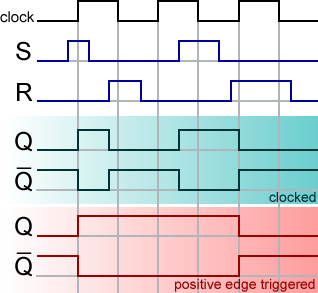
\includegraphics[width=27ex]{SR_FF_timing_diagram.png}}}%^^A
%       \endminipage%
%       \hfill
%       \minipage[c]{\wd\examplecodebox}
%         \hbox{\usebox{\examplecodebox}}
%       \endminipage%
%       }
%     \endgroup
%     \par
%   }%^^A
%   }{}%^^A
% \fi
% \begin{examplecode}
%   \definecolor{bgblue}{rgb}{0.41961,0.80784,0.80784}%
%   \definecolor{bgred}{rgb}{1,0.61569,0.61569}%
%   \definecolor{fgblue}{rgb}{0,0,0.6}%
%   \definecolor{fgred}{rgb}{0.6,0,0}%
%   \begin{tikztimingtable}[timing/slope=0,
%     timing/coldist=2pt,xscale=2.05,yscale=1.1,semithick]
%     \scriptsize clock & 7{C}\\
%     S & .75L h 2.25L H LLl [fgblue]\\
%     R & 1.8L .8H 2.2L 1.4H 0.8L [fgblue]\\
%     Q & L .8H 1.7L 1.5H LL\\
%     $\overline{\mbox{Q}}$ & H .8L 1.7H 1.5L HH\\
%     Q & LHHHHLL[fgred]\\
%     $\overline{\mbox{Q}}$ & HLLLLHH[fgred]\\
%   \extracode
%    \makeatletter
%    \begin{pgfonlayer}{background}
%     \shade [right color=bgblue,left color=white]
%        (7,-8.45) rectangle (-1,-4.6);
%     \shade [right color=bgred,left color=white]
%        (7,-12.8) rectangle (-1,-8.6);
%     \begin{scope}[gray,semitransparent,semithick]
%       \horlines{}
%       \foreach \x in {1,...,6}
%         \draw (\x,1) -- (\x,-12.8);
%       % similar: \vertlines{1,...,6}
%     \end{scope}
%     \node [anchor=south east,inner sep=0pt]
%       at (7,-8.45) {\tiny clocked};
%     \node [anchor=south east,inner sep=0pt,fgred]
%       at (7,-12.8) {\tiny positive edge triggered};
%    \end{pgfonlayer}
%   \end{tikztimingtable}%
% \end{examplecode}
% \caption[SR flip-flop timing diagram]{SR flip-flop timing diagram\texta.  
% Redrawn from image\textb\\ {\small
% \url{http://commons.wikimedia.org/wiki/File:SR_FF_timing_diagram.png}
% }}
% \end{example}
%
% \begin{example}
% \centering
% \lstset{basicstyle=\ttfamily\scriptsize}
% \begin{examplecode}
%   \begin{tikztimingtable}[
%      timing/d/background/.style={fill=white},
%      timing/lslope=0.2,
%      timing/counter/new={char=Q,reset char=R},
%     ]
%             CPOL=0 & LL 15{T} LL \\
%             CPOL=1 & HH 15{T} HH \\
%                    & H 17L H     \\
%     \\
%           Cycle \# & U     R 8{2Q} 2U    \\
%               MISO & D{z}  R 8{2Q} 2D{z} \\
%               MOSI & D{z}  R 8{2Q} 2D{z} \\
%     \\
%           Cycle \# & UU    R 8{2Q} U    \\
%               MISO & D{z}U R 8{2Q} D{z} \\
%               MOSI & D{z}U R 8{2Q} D{z} \\
%   \extracode
%     % Add vertical lines in two colors
%     \begin{pgfonlayer}{background}
%       \begin{scope}[semitransparent,semithick]
%         \vertlines[red]{2.1,4.1,...,17.1}
%         \vertlines[blue]{3.1,5.1,...,17.1}
%       \end{scope}
%     \end{pgfonlayer}
%     % Add big group labels
%     \begin{scope}
%       [font=\sffamily\Large,shift={(-6em,-0.5)},anchor=east]
%       \node at (  0, 0) {SCK};    \node at (  0,-3 ) {SS};
%       \node at (1ex,-9) {CPHA=0}; \node at (1ex,-17) {CPHA=1};
%     \end{scope}
%   \end{tikztimingtable}%
% \end{examplecode}
% \caption[SPI Interface Timing]{SPI Interface Timing.  Redrawn from 
% image {\small
% \url{http://en.wikipedia.org/wiki/File:SPI_timing_diagram.svg}}}
% \end{example}
%
% \clearpage
% \StopEventually{}
% \clearpage
% \iffalse
%</doc>
% \fi
%
%
% \chapter{Implementation}
%
% \subsection{Package Header}
% \iffalse
%<@tikz-timing.sty>
% \fi
%
% \subsection{Libraries}
%
% \subsubsection{Either High or Low}
% \iffalse
%<@tikz-timing-either.sty>
% \fi
%
% \subsubsection{Clock Arrows}
% \iffalse
%<@tikz-timing-clockarrows.sty>
% \fi
%
% \subsubsection{Arrows}
% \iffalse
%<@tikz-timing-arrows.sty>
% \fi
%
% \subsubsection{Overlays}
% \iffalse
%<@tikz-timing-overlays.sty>
% \fi
%
% \subsubsection{Column Type}
% \iffalse
%<@tikz-timing-columntype.sty>
% \fi
%
% \subsubsection{Nice Timing Tables}
% \iffalse
%<@tikz-timing-nicetabs.sty>
% \fi
%
% \subsubsection{Counters}
% \iffalse
%<@tikz-timing-counters.sty>
% \fi
%
% \subsubsection{Advanced Nodes}
% \iffalse
%<@tikz-timing-advnodes.sty>
% \fi
%
% \subsubsection{Intervals}
% \iffalse
%<@tikz-timing-interval.sty>
% \fi
%
% \subsubsection{Beamer Overlay Support}
% \iffalse
%<@tikz-timing-beamer.sty>
% \fi
%
% \subsubsection{Compatibility with \protect\pkg{ifsym} Macros}
% \iffalse
%<@tikz-timing-ifsym.sty>
% \fi
%
%
% \Finale
% \endinput
